\setchapterpreamble[u]{\margintoc} 
\chapter{Analyser et valider les performances d'un système} 
\section{Réaliser une analyse structurelle, flux, effort} 
\graphicspath{{\repStyle/png/}{../SYS/SYS-01/SYS-01_ChaineFonctionnelle/58_Oz440/images/}} 
\normaltrue \difficilefalse \tdifficilefalse
\correctiontrue

%\UPSTIidClasse{11} % 11 sup, 12 spé
%\newcommand{\UPSTIidClasse}{12}
% CCP MP 2016
\exer{Robot de maraîchage Oz 440 $\star$ \label{SYS:01:58}}
\setcounter{question}{0}
\marginnote[5cm]{\xpComp{SYS}{01}}
\index{Compétence SYS-01}
\index{Robot de maraîchage Oz 440 }
\index{Associer les fonctions aux constituants.}

\ifcorrection
\else
\marginnote{\textbf{Pas de corrigé pour cet exercice.}}
\fi

\ifprof
\else

Le robot de maraîchage Oz 440 développé par la société Naïo Technologies est un outil autonome
agricole, alliant robustesse et écologie, capable d’assister les maraîchers dans les tâches les plus
pénibles comme le transport de charges lors des récoltes et le désherbage mécanique à l’aide d’un
outil de binage.


\begin{marginfigure}[5cm]
\centering
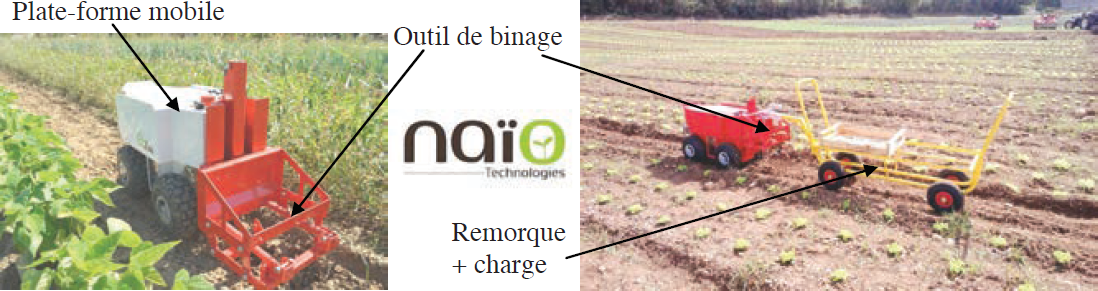
\includegraphics[width=\linewidth]{58_01}
%\caption{Amplificateur de charge à plusieurs canaux KISTLER. \label{fig_50_01}}
\end{marginfigure}


Ce robot est constitué d’une plate-forme mobile électrique à 4 roues motrices sur laquelle sont
fixés divers outils et capteurs. La figure 1 donne la structure du robot sous la forme d’un
diagramme de définition de blocs (BDD) avec les propriétés principales de chaque constituant,
utiles pour la résolution du problème.

\begin{figure}[H]
\centering
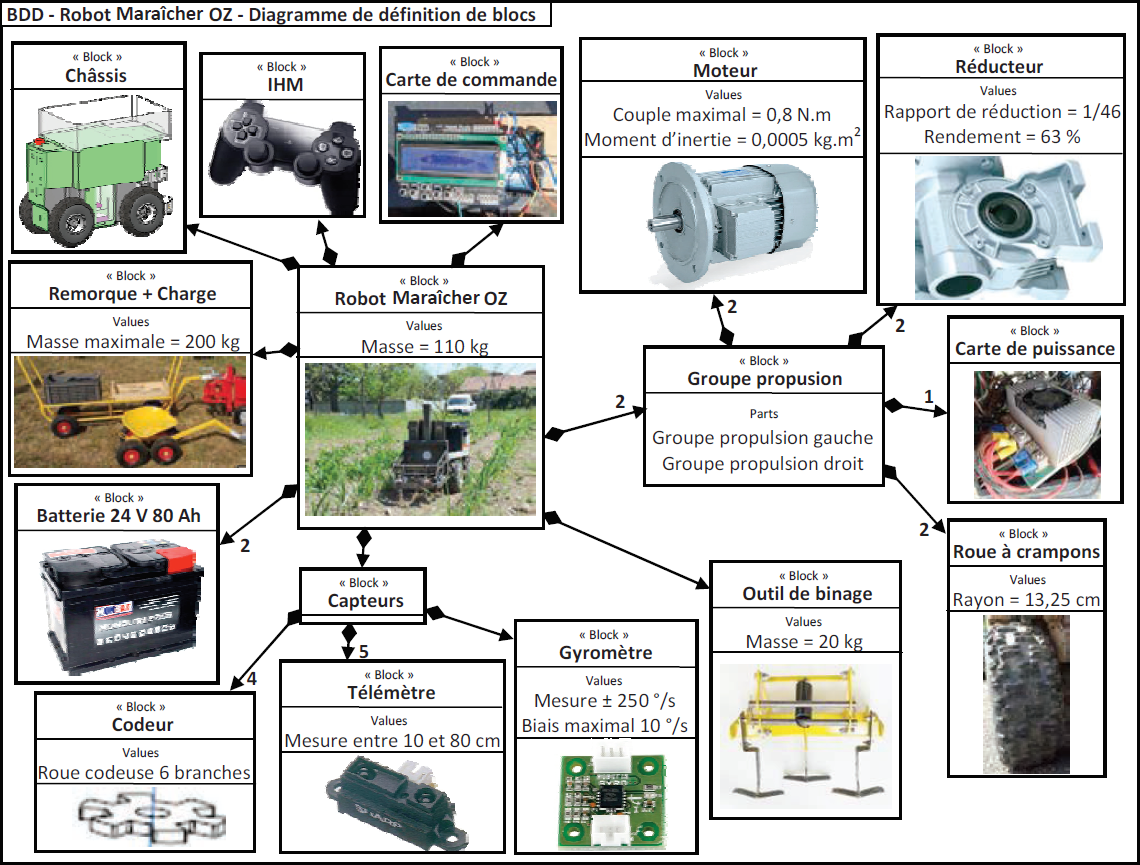
\includegraphics[width=\linewidth]{58_02}
%\caption{Amplificateur de charge à plusieurs canaux KISTLER. \label{fig_50_01}}
\end{figure}


Ce robot de petite taille évolue directement entre les rangées de cultures pour un travail de
précision. Il peut, par exemple, désherber et aussi suivre des personnes lors de la récolte tout en
transportant des charges. Bien plus petit qu’un tracteur classique, il ne casse pas la structure
naturelle du sol et évite ainsi le phénomène de compaction des sols provoqué habituellement par les
tracteurs ou le piétinement de l’homme. Il roule lentement et passe au plus près des cultures sans
risquer de les abîmer. Selon le vieil adage « un binage vaut deux arrosages », le fait de pouvoir
utiliser ce robot régulièrement, sans perte de temps, permet de toujours avoir un sol parfaitement
biné et ainsi de diminuer les effets d’évaporation de l’eau.
\fi

\question{À l’aide du diagramme de définition de blocs disponible, réaliser le diagramme correspondant à la chaîne fonctionnelle de l’ensemble
groupe propulsion droit du robot.}
\ifprof

\begin{figure}[H]
\centering
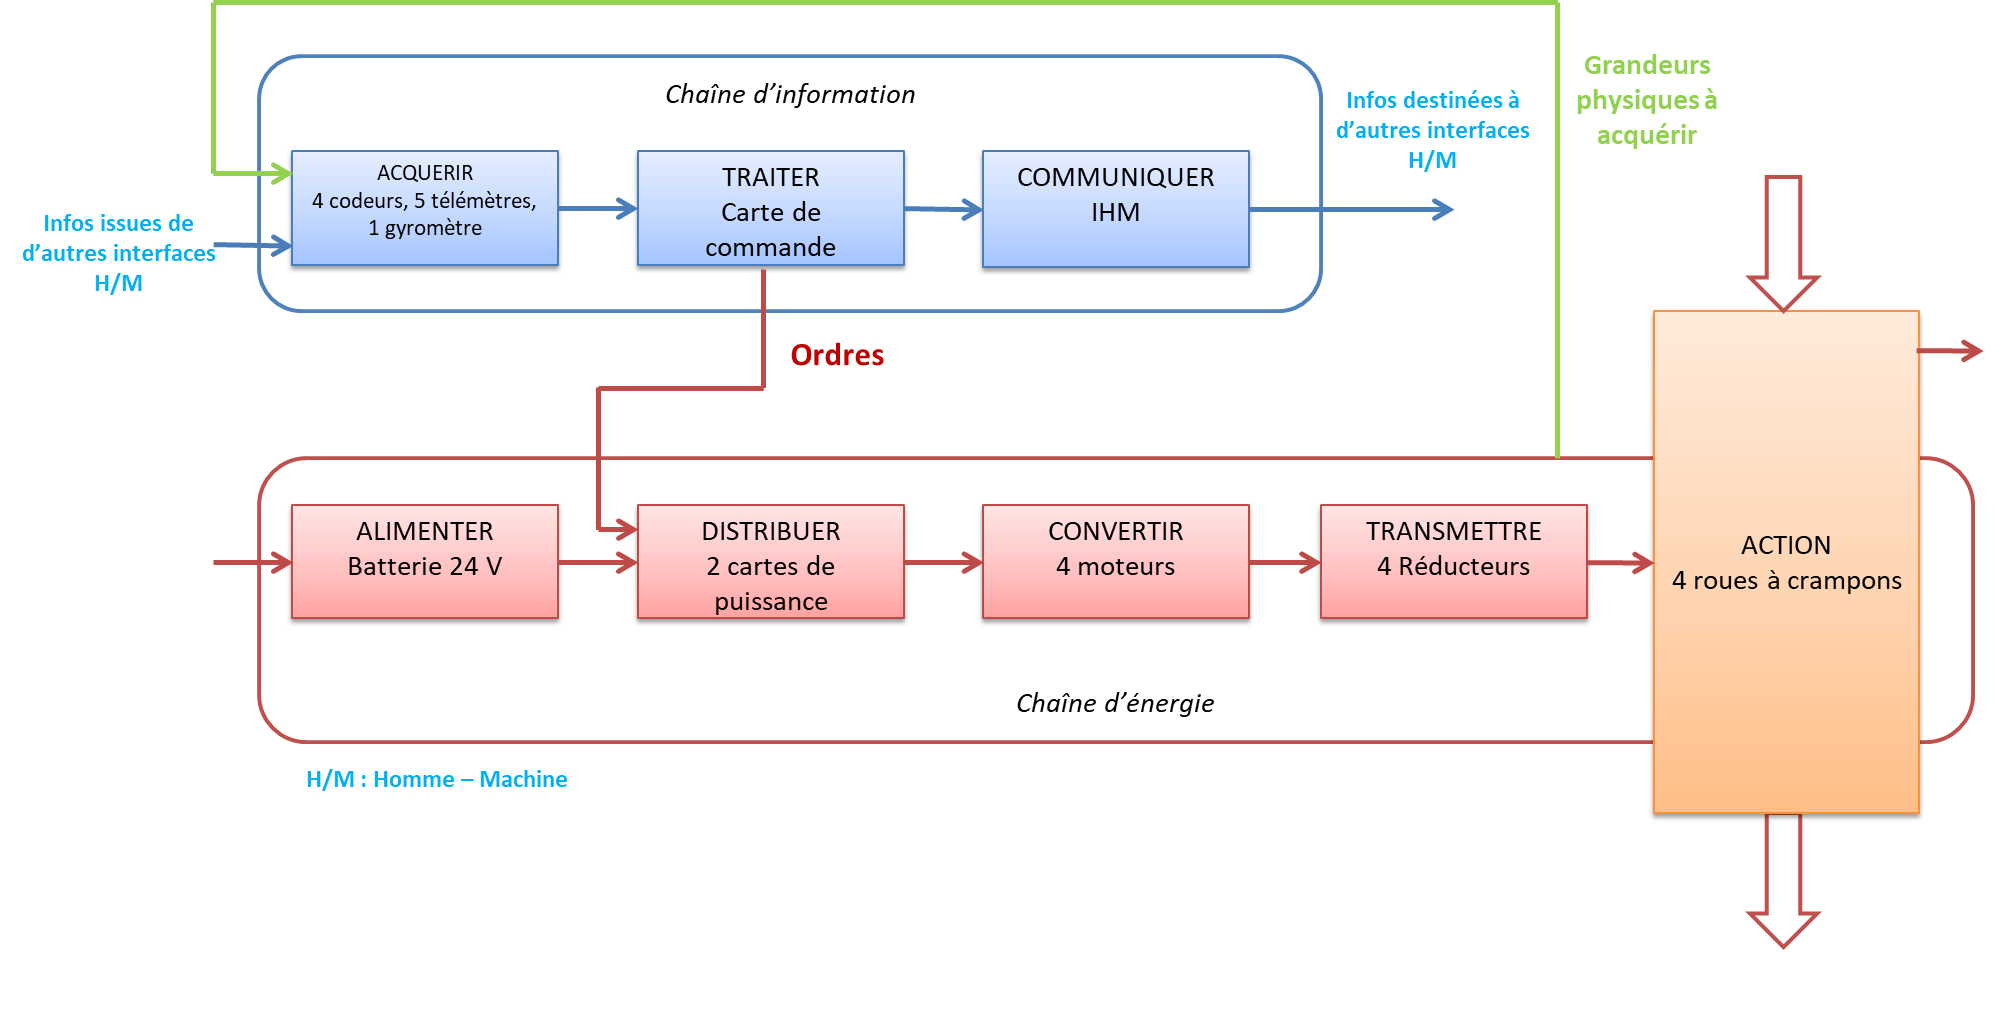
\includegraphics[width=\linewidth]{58_01_cor}
%\caption{Amplificateur de charge à plusieurs canaux KISTLER. \label{fig_50_01}}
\end{figure}

\else

\marginnote{Corrigé  voir \ref{SYS:01:58}.}

\fi 
 
\graphicspath{{\repStyle/png/}{../SYS/SYS-01/SYS-01_ChaineFonctionnelle/59_Levage/images/}} 
\normaltrue \difficilefalse \tdifficilefalse
\correctionfalse

%\UPSTIidClasse{11} % 11 sup, 12 spé
%\newcommand{\UPSTIidClasse}{12}
% CCP MP 2011
\exer{Système de levage à multiples colonnes $\star$ \label{SYS:01:59}}
\setcounter{question}{0}\marginnote{\xpComp{SYS}{01}}
\index{Compétence SYS-01}
\index{Système de levage à multiples colonnes }
\index{Associer les fonctions aux constituants.}

\ifcorrection
\else
\marginnote{\textbf{Pas de corrigé pour cet exercice.}}
\fi

\ifprof
\else

Les sociétés de transports publics des grandes agglomérations gèrent des réseaux comportant des
bus et/ou des tramways. Ces sociétés possèdent des centres de maintenance ayant en charge
l’entretien et la réparation de leurs véhicules. %Parmi ces véhicules, on peut trouver des tramways de
%deux types : sur rails ou sur pneus. 
On s'intéresse ici à la maintenance de tramways sur rails de type
TFS (Tramway Français Standard).


Le système de levage est constitué d’une armoire de commande (nommée PC) munie d’un pupitre
de commande, d’un API (Automate Programmable Industriel), de relais et cartes de commande
pour moteurs. Cette PC peut gérer jusqu’à 10 colonnes de levage. Ces colonnes de levage sont des unités indépendantes mobiles que l’on peut déplacer manuellement
grâce à des roues escamotables. Elles sont constituées d’un chariot de levage guidé par 4 galets roulant à l’intérieur d’une colonne (rails
en tôle pliée). 


L’entraînement du chariot se fait par une vis à filet trapézoïdal, mise en rotation par un moto-réducteur-frein asynchrone. On met en place les colonnes au
niveau de la plate forme du tramway à soulever, aux endroits prévus à cet effet.


%\begin{multicols}{2}
\begin{marginfigure}
\centering
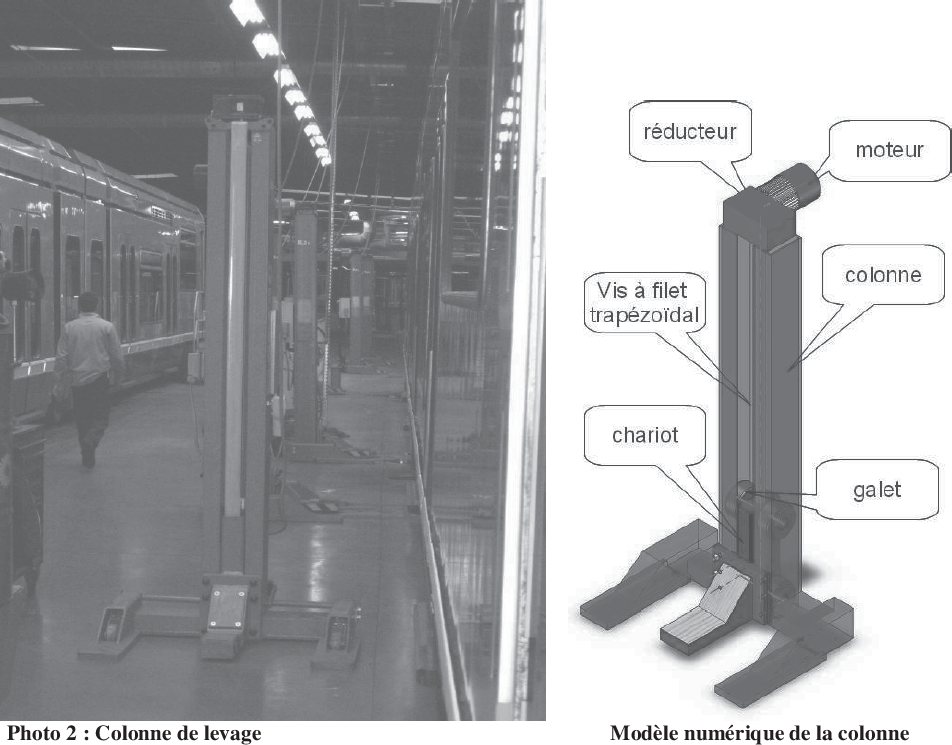
\includegraphics[width=\linewidth]{59_01}
%\caption{Amplificateur de charge à plusieurs canaux KISTLER. \label{fig_50_01}}
\end{marginfigure}

\begin{marginfigure}
\centering
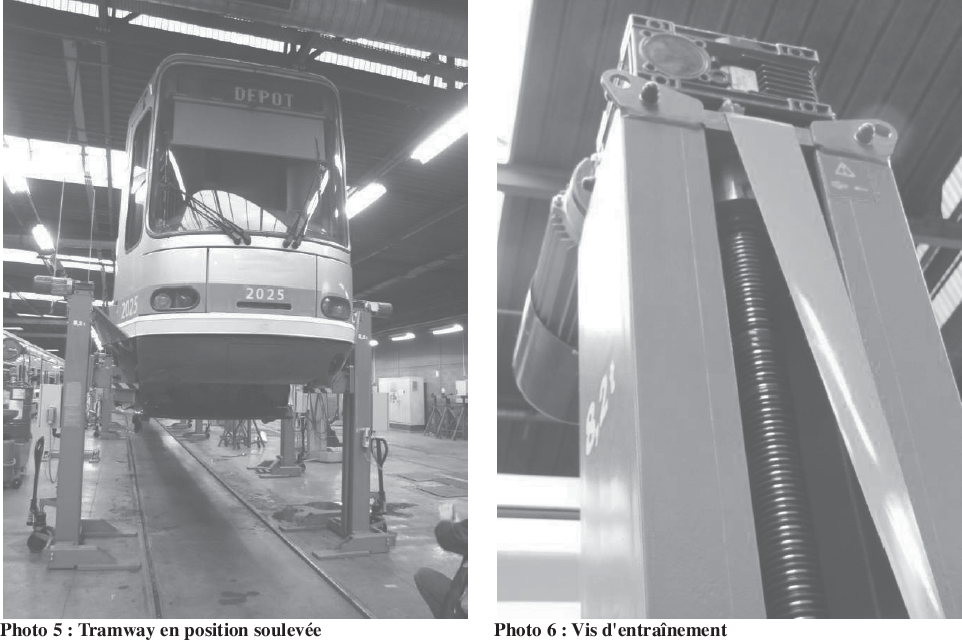
\includegraphics[width=\linewidth]{59_02}
\end{marginfigure}

%\end{multicols}

Pour soulever un tramway de \SI{45}{tonnes} et de 30 mètres de long, le service de maintenance utilise 8
colonnes de levage d'une capacité unitaire maximale de 8,2 tonnes commandées simultanément. Lorsque les colonnes sont en place, on démarre le cycle de levage :
l’opérateur peut choisir un fonctionnement manuel ou automatique. En mode automatique, on
affiche sur le pupitre la consigne de hauteur à atteindre, la PC pilote alors chaque moteur des 8
colonnes jusqu’à ce que cette hauteur soit atteinte. Chaque colonne est équipée d’un codeur
incrémental informant la PC de la position du chariot de levage de la colonne. Pour un
fonctionnement en toute sécurité, il faut assurer une certaine horizontalité du tramway soulevé :
l'ensemble des points de levage doit être compris entre deux plans parallèles distants de \SI{20}{mm} au
maximum (coplanéité).

Le développement sous forme de FAST de la fonction principale F.P.1 (plus simplement écrite
« Soulever un tramway ») est donné ci-après.

\begin{marginfigure}
\centering
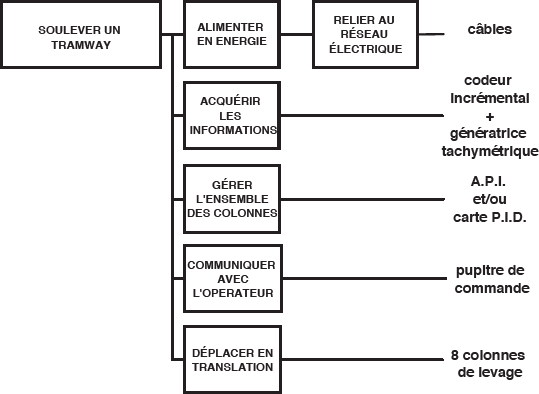
\includegraphics[width=\linewidth]{59_03}
\end{marginfigure}

Le développement sous forme de FAST de la fonction technique « Déplacer en translation » pour
une colonne est donné ci-après.

\begin{marginfigure}
\centering
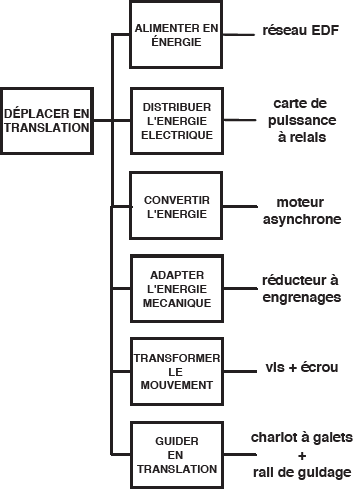
\includegraphics[width=\linewidth]{59_04}
\end{marginfigure}


\fi

\question{Vous ne connaissez pas le diagramme FAST (je le sais). Quel(s) diagramme(s) SysML pourriez-vous utiliser pour remplacer les diagrammes <<~FAST~>>.}

\question{Réaliser la chaîne fonctionnelle du système de levage étudié.}


\ifprof
\else

\marginnote{Corrigé  voir \ref{SYS:01:59}.}

\fi 
 
\graphicspath{{\repStyle/png/}{../SYS/SYS-01/SYS-01_ChaineFonctionnelle/60_Escalier/images/}} 
\normaltrue \difficilefalse \tdifficilefalse
\correctionfalse

%\UPSTIidClasse{11} % 11 sup, 12 spé
%\newcommand{\UPSTIidClasse}{12}
% CCP MP 2014
\exer{Escalier mécanique$\star$ \label{SYS:01:60}}
\setcounter{question}{0}\marginnote{\xpComp{SYS}{01}}
\index{Compétence SYS-01}
\index{Escalier mécanique}
\index{Associer les fonctions aux constituants.}

\ifcorrection
\else
\marginnote{\textbf{Pas de corrigé pour cet exercice.}}
\fi

\ifprof
\else


Un escalier mécanique (figure 1), appelé aussi escalier roulant ou Escalator (nom déposé par la société Otis), est un élévateur adapté au transport de personnes. Sa fonction principale est de faciliter le déplacement des piétons entre deux points de différentes hauteurs. 

%Depuis son invention en 1892 (à New York) par l’américain Jesse W. Reno, le système n’a pas cessé d’évoluer pour s’adapter aux nouvelles contraintes économiques, environnementales et sécuritaires.


\begin{marginfigure}
\centering
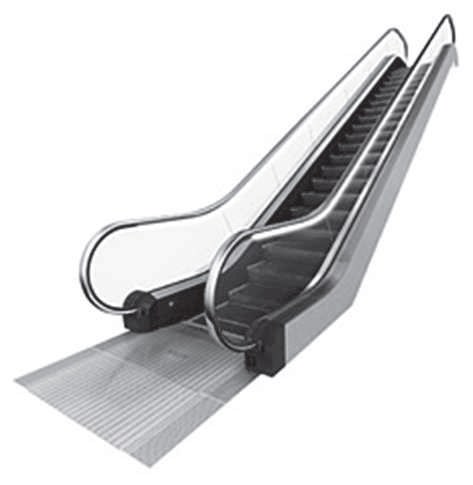
\includegraphics[width=4cm]{60_01}
%\caption{Amplificateur de charge à plusieurs canaux KISTLER. \label{fig_50_01}}
\end{marginfigure}

%\ifprof
%\else
%\end{multicols}
\begin{figure}[H]
\centering
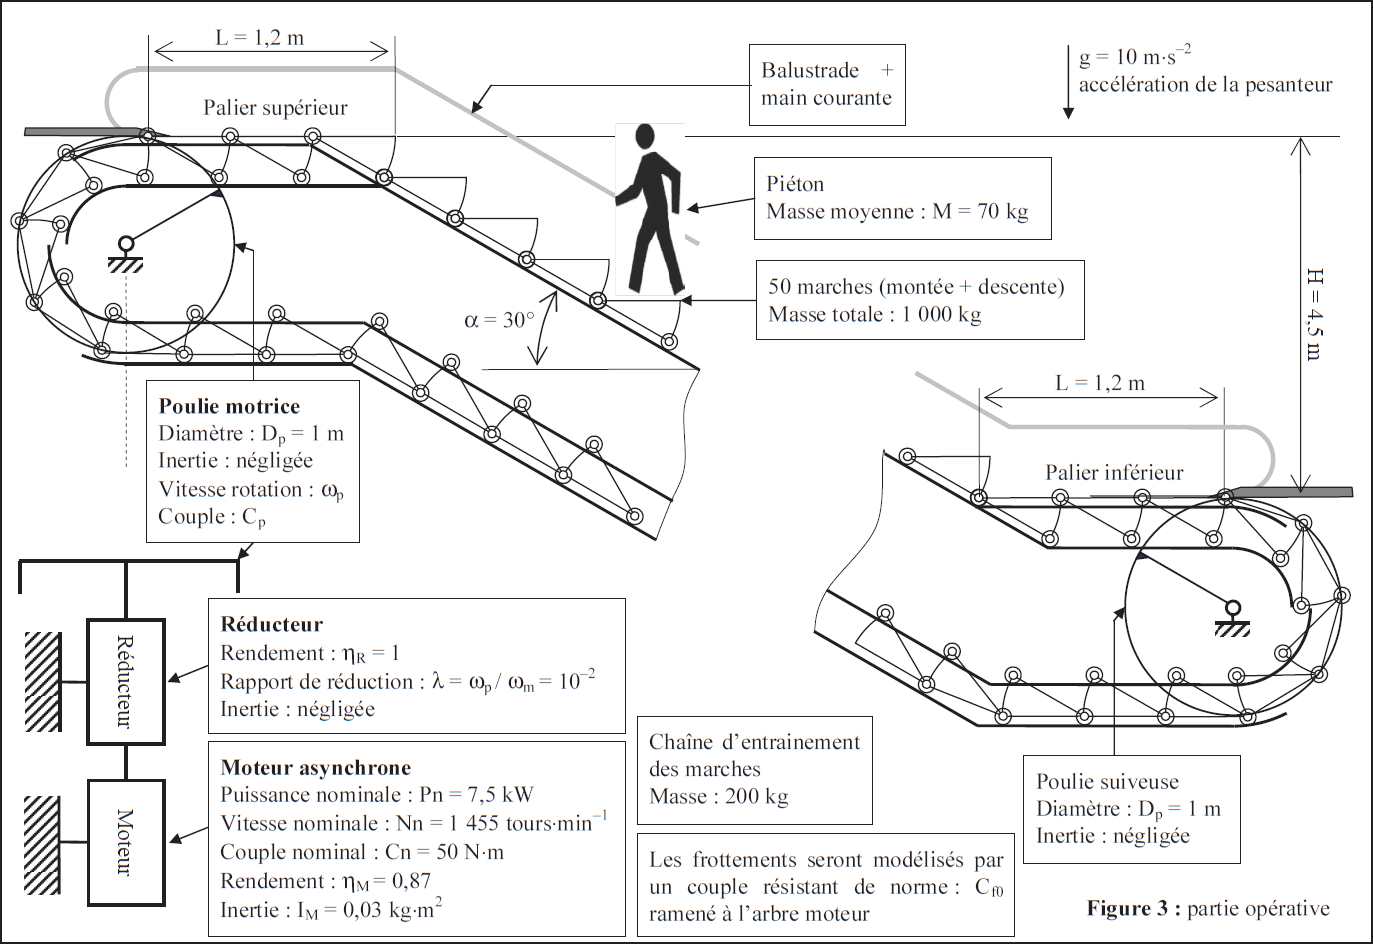
\includegraphics[width=\linewidth]{60_02}

\end{figure}
%\begin{multicols}{2}
\fi


\question{En analysant le schéma de principe de la figure précédente, proposer une chaîne fonctionnelle de l'escalier mécanique.}


\ifprof
\else
\begin{flushright}
\footnotesize{Corrigé  voir \ref{SYS:01:60}.}
\end{flushright}%
\fi 
 
\graphicspath{{\repStyle/png/}{../SYS/SYS-01/SYS-01_ChaineInfo/507_Divers/images/}} 
\normaltrue \difficilefalse \tdifficilefalse
\correctionfalse

%\UPSTIidClasse{11} % 11 sup, 12 spé
%\newcommand{\UPSTIidClasse}{12}
% ATS 2019
\exer{Capteurs $\star$ \label{SYS:01:507}}
\setcounter{question}{0}\marginnote{\xpComp{SYS}{01}}
\index{Compétence SYS-01}
\index{Caractériser un constituant de la chaîne d’information.}
\index{Capteurs}
\ifcorrection
\else
\marginnote{\textbf{Pas de corrigé pour cet exercice.}}
\fi


\question{Donner le rôle et le principe de fonctionnement (schémas) des capteurs suivants : 
\begin{itemize}
\item génératrice tachymétrique;
\item potentiomètre rotatif;
\item codeur incrémental ;
\item codeur absolu. 
\end{itemize}.}
\ifprof
\else
\fi




\ifprof
\else

\marginnote{Corrigé voir \ref{SYS:01:507}.}

\fi 
 
\graphicspath{{\repStyle/png/}{../SYS/SYS-01/SYS-01_ChaineInfo/50_BancBalafre/images/}} 
\normaltrue \difficilefalse \tdifficilefalse
\correctionfalse

%\UPSTIidClasse{11} % 11 sup, 12 spé
%\newcommand{\UPSTIidClasse}{12}
% ATS 2019
\exer{Le banc balafre $\star$ \label{SYS:01:50}}
\setcounter{question}{0}\marginnote{\xpComp{SYS}{01}}
\index{Compétence SYS-01}
\index{Le Banc Balafre}
\index{Caractériser un constituant de la chaîne d’information.}
\index{Capteurs}
\ifcorrection
\else
\marginnote{\textbf{Pas de corrigé pour cet exercice.}}
\fi

\ifprof
\else


Entre autres contrôles de la chaîne d’acquisition, le superviseur vérifie que la mesure des efforts se fait correctement : au niveau des actionneurs piézoélectriques et au niveau du joint testé. Les capteurs de force utilisés sur le système sont analogiques. Afin de simplifier le traitement et l’interprétation de ces forces, on utilise un amplificateur de charges à plusieurs canaux (voir figure \ref{fig_50_01}).


\begin{marginfigure}
\centering
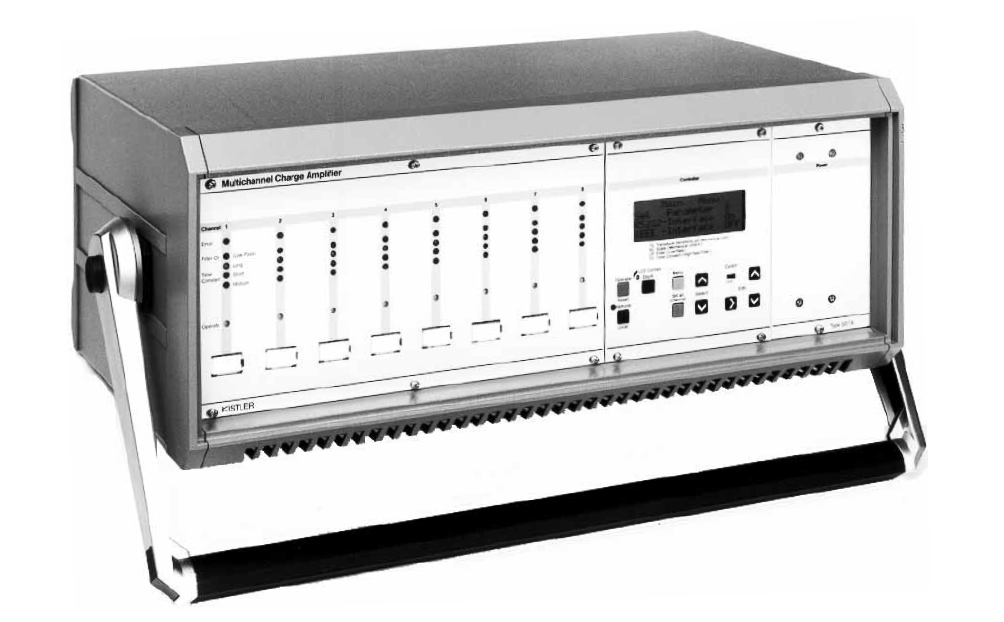
\includegraphics[width=\linewidth]{fig_50_01}
\caption{Amplificateur de charge à plusieurs canaux KISTLER. \label{fig_50_01}}
\end{marginfigure}



Cet amplificateur possède deux options qui sont utilisées sur le banc Balafre :
\begin{itemize}
\item l’amplificateur de sommation pour le calcul analogique des forces et moments résultants
;
\item un convertisseur Analogique/Numérique pour faire le traitement des données (algorithme
de contrôle).
\end{itemize}
Dans l’algorithme de contrôle, la valeur d’effort de chaque actionneur est comparée à
la valeur théorique de la consigne effectuée pour le contrôle. Si un écart trop grand est
constaté, l’algorithme de contrôle émet un signal d’erreur (Controle=2). Pour cette mesure,
on considère qu’une résolution inférieure à  \SI{10}{N} est nécessaire.
La conversion analogique/numérique se fait ici sur 12 bits. La mesure de l’effort se fait
sur la plage de $-20$ à \SI{20}{kN}. Les données techniques utiles sont rassemblées sur la figure
\ref{fig_50_02}.

\begin{marginfigure}
\centering
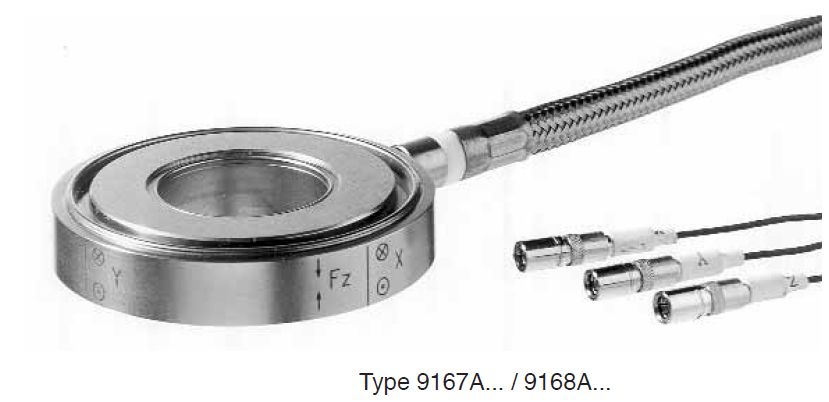
\includegraphics[width=.7\linewidth]{fig_50_03}
\caption{Capteur de force KISTLER 9167A. \label{fig_50_03}}
\end{marginfigure}

Le capteur de force (voir figure \ref{fig_50_03}) utilisé est un capteur KISTLER 9167A, permettant
de mesurer des efforts dans trois directions. Pour la mesure de l’effort développé par
les actionneurs, seule la direction Z est utilisée, et la sensibilité du capteur dans cette
direction est \SI{4,2}{pC.N^{-1}}.
Le synoptique de la figure \ref{fig_50_04} présente la structure interne de l’amplificateur de charge.

\begin{figure}[H]
\centering
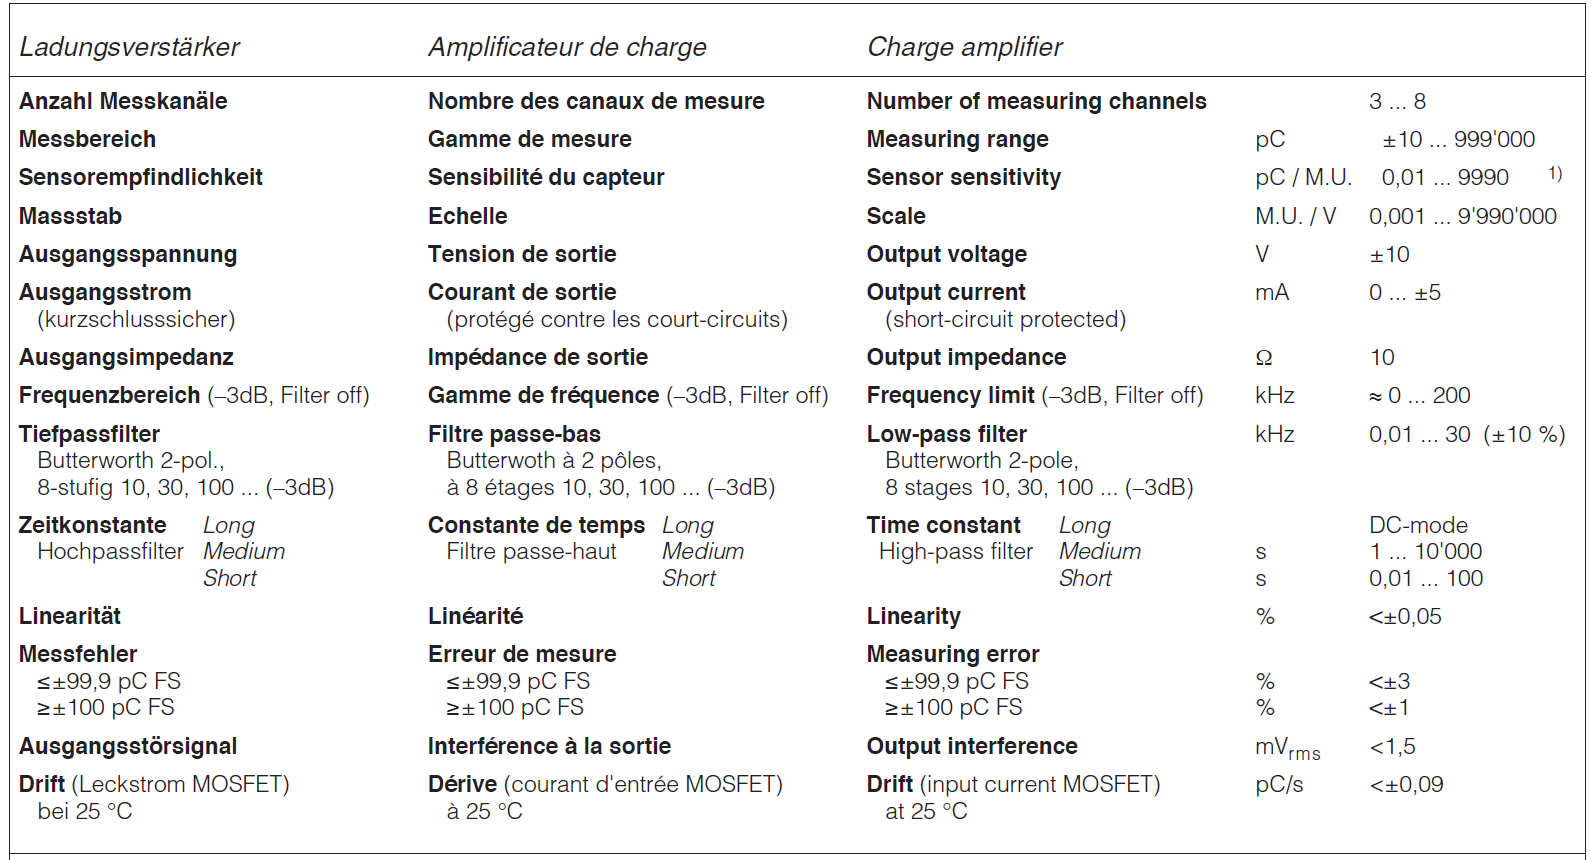
\includegraphics[width=\linewidth]{fig_50_02}
\caption{Amplificateur de charge à plusieurs canaux KISTLER. \label{fig_50_02}}
\end{figure}



\begin{figure}[H]
\centering
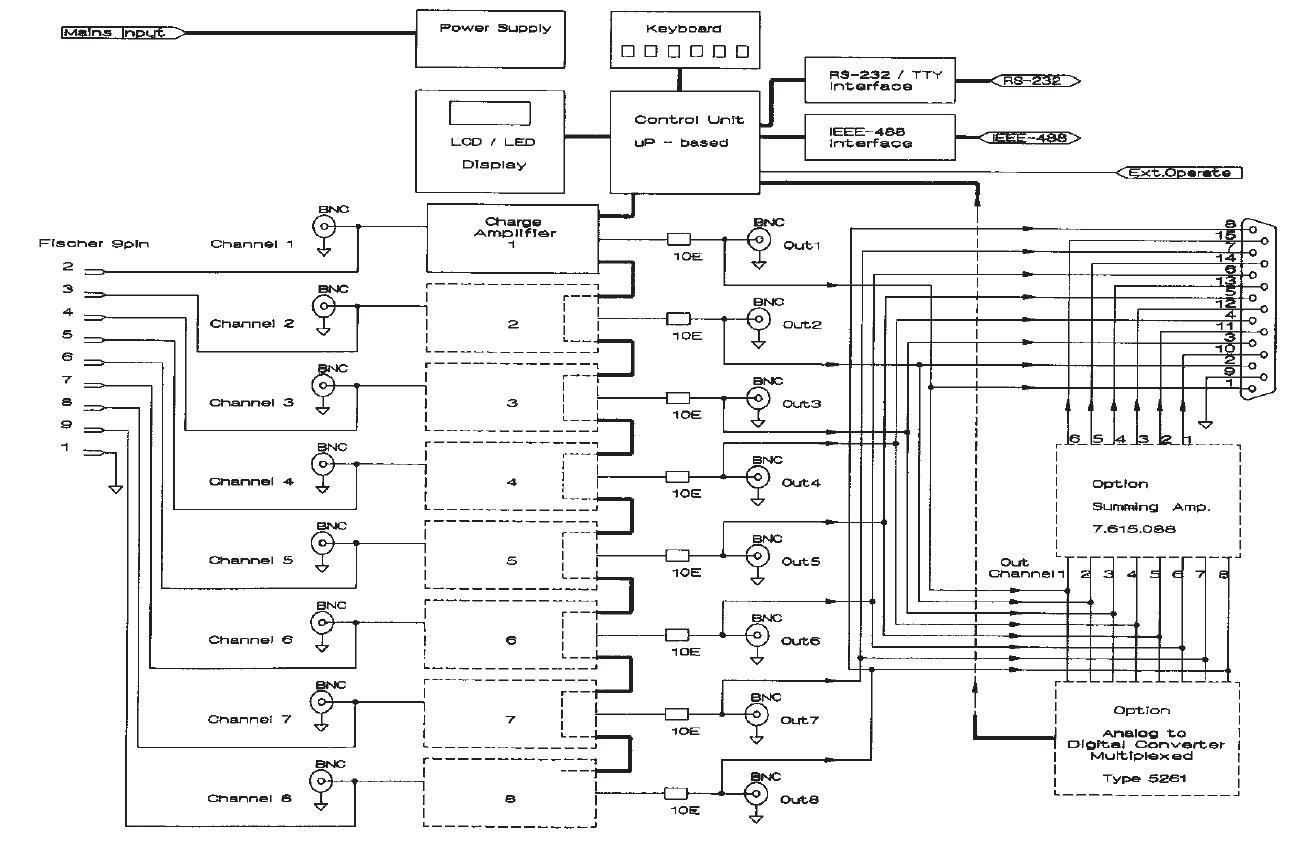
\includegraphics[width=\linewidth]{fig_50_04}
\caption{Synoptique de la structure interne de l’amplificateur de charge. \label{fig_50_04}}
\end{figure}
\fi

\question{Sur le synoptique de la figure \ref{fig_50_04}, on peut lire « Analog to Digital Converter Multiplexed ». Que signifie le terme multiplexé utilisé ici ?}
\ifprof
\else
\fi

\question{Compte tenu de la sensibilité du capteur et de l’étendue des valeurs à
mesurer, déterminer la gamme de mesure à régler sur l’amplificateur de charge.}
\ifprof
\else
\fi

\question{En utilisant la documentation technique de l’amplificateur de charge,
déterminer la plage de variation de la tension de sortie de l’amplificateur. En déduire le
quantum de la conversion analogique numérique, puis la résolution de la mesure. Conclure
vis-à-vis de la résolution demandée.}
\ifprof
\else
\fi




\ifprof
\else

\marginnote{Corrigé  voir \ref{SYS:01:50}.}

\fi 
 
\graphicspath{{\repStyle/png/}{../SYS/SYS-01/SYS-01_ChaineInfo/538_Codeur/images/}} 
\normaltrue \difficilefalse \tdifficilefalse
\correctionfalse

%\UPSTIidClasse{11} % 11 sup, 12 spé
%\newcommand{\UPSTIidClasse}{12}
% ATS 2019
\exer{Codeur incrémental $\star$ \label{SYS:01:538}}
\setcounter{question}{0}\marginnote{\xpComp{SYS}{01}}
\index{Compétence SYS-01}
\index{Caractériser un constituant de la chaîne d’information.}
\index{Capteurs}
\ifcorrection
\else
\marginnote{\textbf{Pas de corrigé pour cet exercice.}}
\fi

\begin{marginfigure}
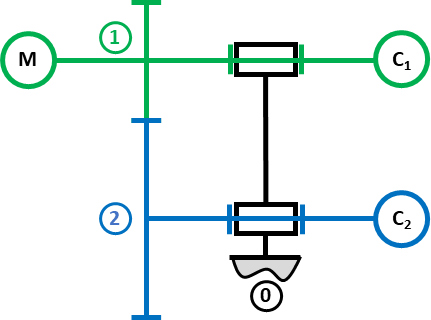
\includegraphics[width=5cm]{538_01}
\end{marginfigure}

\question{Donner le rôle et le principe de fonctionnement (schémas) d'un codeur incrémental optique.}
\ifprof
\else
\fi

\question{Le codeur est équipé d'une voie de mesure et d'un disque à 25 fentes. Donner la résolution du capteur en degtés.}
\ifprof
\else
\fi

\question{Quelle sera la résolution du capteur s'il est équipé de deux voies de mesure ?}
\ifprof
\else
\fi

\ifprof
\else
Un codeur est monté en sortie d'un moteur. Le moteur est suivi d'un réducteur de rapport 100.

\fi

\question{Quelle est la résolution du capteur vis-à-vis de l'arbre de sortie du réducteur ?}
\ifprof
\else
\fi

\ifprof
\else
La position du codeur est transformée par un convertisseur numérique analogique en V. Ce convertisseur permet de convertir des angles variants de $-$10 tours à +10 tours sur une échelle de $-5$ à +\SI{5}{V}.   
\fi

\question{Donner le gain du convertisseur numérique analogique.}
\ifprof
\else
\fi


\ifprof
\else

\marginnote{Corrigé  voir \ref{SYS:01:538}.}

\fi 
 
\graphicspath{{\repStyle/png/}{../SYS/SYS-01/SYS-01_ChainePuissance/1100_Pneumatique/images/}} 
\normaltrue \difficilefalse \tdifficilefalse
\correctionfalse

%\UPSTIidClasse{11} % 11 sup, 12 spé
%\newcommand{\UPSTIidClasse}{12}
% ATS 2019
\exer{Vérin double effets $\star$ \label{A3:05:1100}}
\setcounter{question}{0}\marginnote{\xpComp{SYS}{01}}
\index{Compétence A3-05}
\index{Distributeur}
\index{Vérin}
\ifcorrection
\else
\marginnote{\textbf{Pas de corrigé pour cet exercice.}}
\fi


Un vérin double effet est commandé par un distributeur 4/2 (4 orifices, 2 positions) bi-stable.



\ifprof
\else
%\begin{marginfigure}
%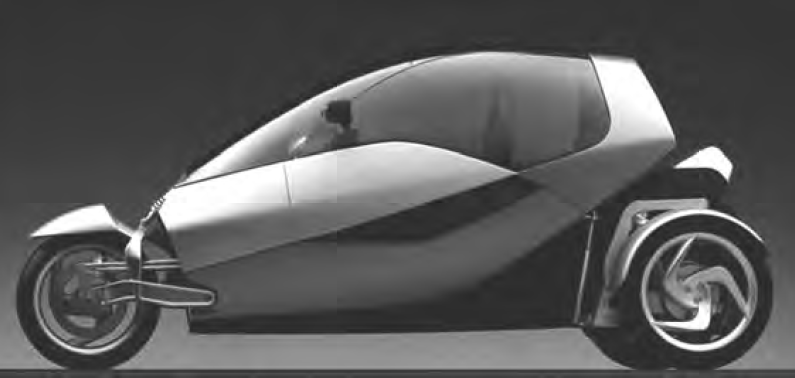
\includegraphics[width=.8\linewidth]{fig_80_01}
%%\textit{}
%\end{marginfigure}




\begin{marginfigure}
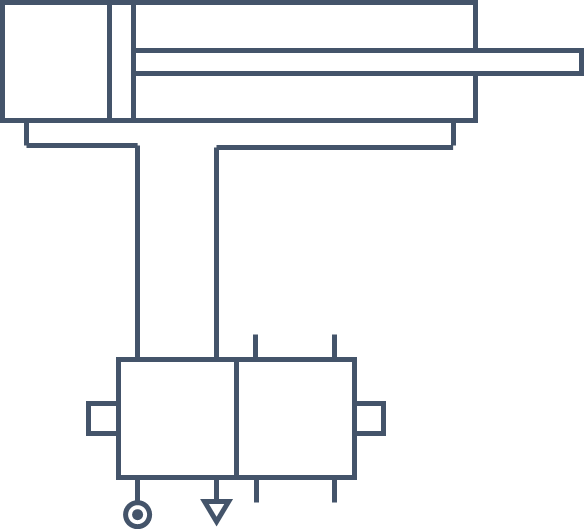
\includegraphics[width=\linewidth]{1100_fig_01}
%\textit{}
\end{marginfigure}

\question{Compléter le câblage du distributeur.}

\question{Dans la position actuelle, indiquer par des flèches le sens de déplacement du vérin. Indiquer en rouge les tuyaux et chambre hautes pressions. Indiquer en bleu les tuyaux et chambre basses pressions.}

\question{On souhaite ralentir le déplacement du vérin lorsqu'il sort de la chambre. Positionner le limiteur de débit en conséquence.}

\begin{marginfigure}
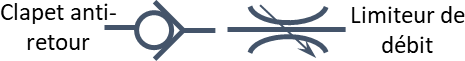
\includegraphics[width=\linewidth]{1100_fig_02}
%\textit{}
\end{marginfigure}


\question{Ajouter un clapet anti-retour pour éviter la limitation du débit lorsque le vérin se rétracte.}



\ifprof
\begin{corrige}
\begin{center}
%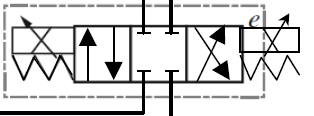
\includegraphics[width=.5\linewidth]{fig_80_cor_01}
%\textit{}
\end{center}
\end{corrige}
\else\begin{center}
%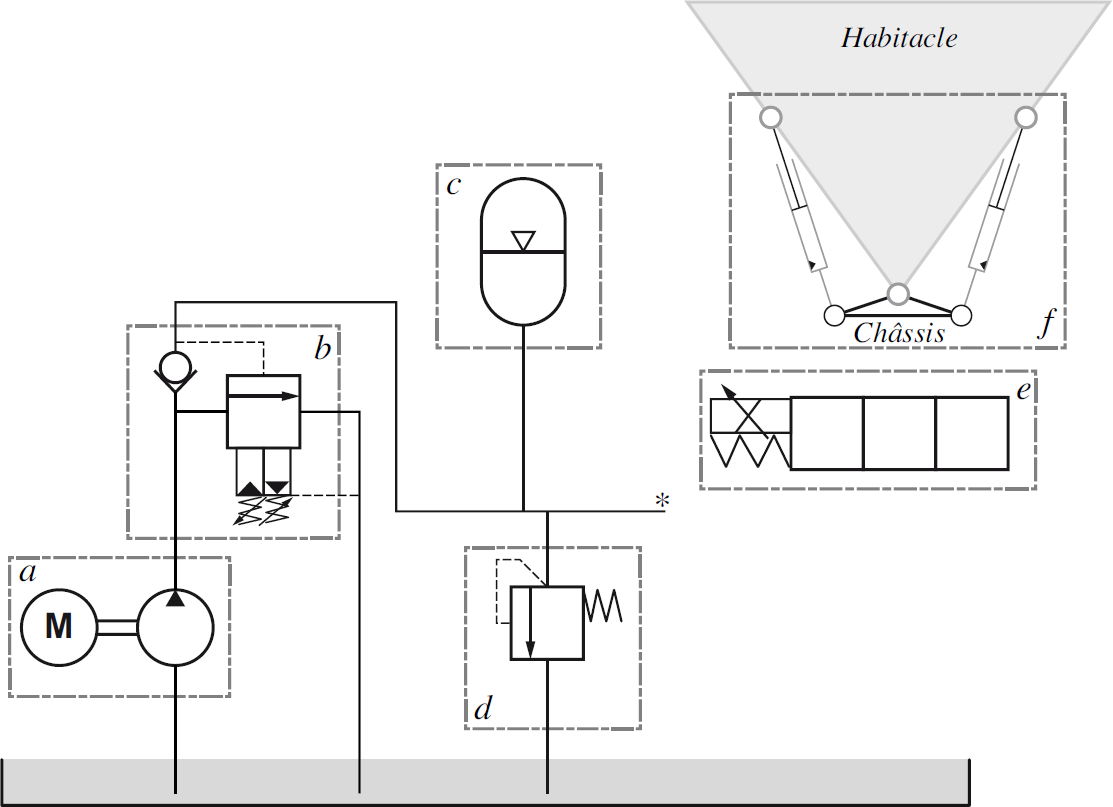
\includegraphics[width=\linewidth]{fig_80_05}
%\textit{}
\end{center}

\fi

Au démarrage du véhicule, la valve de décharge du module (b) est fermée. Le distributeur à effet proportionnel(e) est en position médiane, les vérins sont donc immobiles. La commande des vérins est initialement bloquée par une temporisation.

\question{En considérant les conditions initiales évoquées, expliquer, en commençant à l’instant de démarrage de la pompe, le comportement du circuit hydraulique en précisant clairement les différentes phases de fonctionnement. Quel est l’utilité de la temporisation ? On souhaite remplacer cette temporisation par un capteur. Préciser la grandeur qu’il devra mesurer. Donner un avantage et un inconvénient du remplacement de la temporisation par ce capteur.}
\ifprof
\begin{corrige}
Démarrage de la pompe et montée en pression du circuit avec remplissage de l’accumulateur (c).

À la fin de la temporisation le distributeur peut être commandé et ainsi alimenter les vérins.

Si la pression augmente trop, alors le limiteur de pression (d) renvoie une partie du fluide vers le
réservoir et si c’est insuffisant alors (b) permet une décharge du circuit (ouverture vers le réservoir
jusqu’à atteindre ne niveau bas réglé).

La temporisation permet d’attendre qu’un niveau de pression suffisant dans le circuit soit atteint.

Pour remplacer la temporisation on peut mesurer la pression dans le circuit ou plus simplement détecter
le niveau de pression satisfaisant pour le fonctionnement à l’aide d’un pressostat.

La solution utilisant un capteur de pression est plus sûre que la temporisation qui pourrait autoriser la
commande du distributeur alors que la pression dans le circuit est encore insuffisante.

(UPSTI). 
\end{corrige}
\else
\fi






\ifprof
\else
\begin{flushright}
\footnotesize{Corrigé  voir \ref{A3:05:80}.}
\end{flushright}%
\fi 
 
\graphicspath{{\repStyle/png/}{../SYS/SYS-01/SYS-01_ChainePuissance/80_Clever/images/}} 
\normaltrue \difficilefalse \tdifficilefalse
\correctionfalse

%\UPSTIidClasse{11} % 11 sup, 12 spé
%\newcommand{\UPSTIidClasse}{12}
% ATS 2019
\exer{Véhicule à trois roues Clever $\star$ \label{A3:05:80}}
\setcounter{question}{0}%\marginnote{\xpComp{SYS}{01}}
\marginnote{\index{Compétence A3-05}}
\index{Véhicule à trois roues Clever}
\index{Caractériser un constituant de la chaîne de puissance.}
\index{Distributeur}
\index{Vérin}
\ifcorrection
\else
\marginnote{\textbf{Pas de corrigé pour cet exercice.}}
\fi




On s'intéresse au véhicule à 3 roues Clever.

\ifprof
\else
%\begin{marginfigure}
%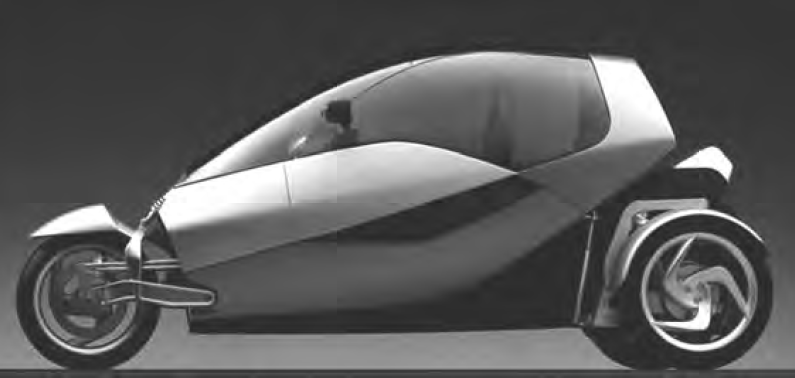
\includegraphics[width=.8\linewidth]{fig_80_01}
%%\textit{}
%\end{marginfigure}


 Le groupe motopropulseur est placé à l'arrière du véhicule. À l’avant, l’habitacle repose sur une roue de moto et pivote par rapport au bloc arrière autour d’une liaison pilotée angulairement par le biais de deux vérins hydrauliques. L'inclinaison est contrôlée par un ordinateur de bord en fonction de l'angle au volant et de la vitesse. 

\begin{marginfigure}
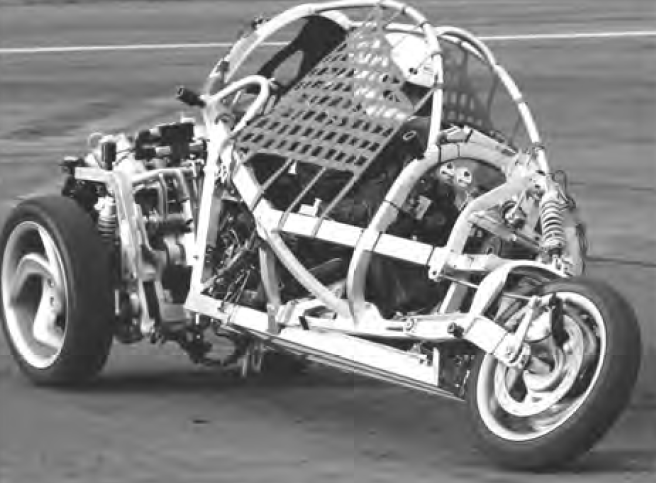
\includegraphics[width=\linewidth]{fig_80_02}
%\textit{}
\end{marginfigure}

%Le système d’inclinaison de l’habitacle est assuré par un système constitué :
%\begin{itemize}
%\item d’un calculateur qui détermine le mouvement et la position à donner à l’habitacle en fonction des conditions
%d’utilisation;
%\item d’un système hydro-mécanique de transmission de puissance et d’adaptation de mouvement;
%\item d’un système de contrôle de l’inclinaison de l’habitacle.
%\end{itemize}

La chaîne de transmission de puissance et d’adaptation de mouvement est composée :
\begin{itemize}
\item d’une pompe à engrenages actionnée par le moteur à gaz via un système de poulies/courroie;
\item d’un circuit hydraulique;
\item de 2 vérins hydrauliques simple effet;
\item d’un système mécanique d’adaptation de mouvement afin de transformer le mouvement de translation des tiges des vérins en rotation de l’habitacle.
\end{itemize}


\begin{center}
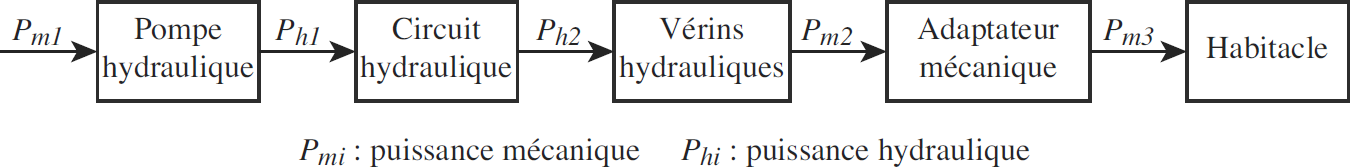
\includegraphics[width=\linewidth]{fig_80_03}
%\textit{}
\end{center}

\begin{center}
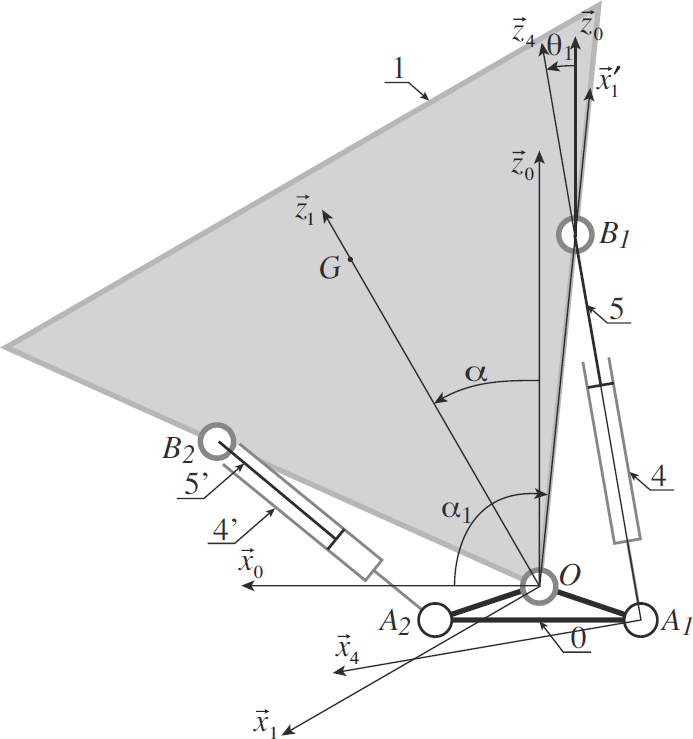
\includegraphics[width=.7\linewidth]{fig_80_04}
%\textit{}
\end{center}


Les deux vérins hydrauliques transforment la puissance hydraulique venant du servo-distributeur afin d’incliner l’habitacle. Ceux-ci sont disposées entre l’habitacle et le châssis du module arrière de propulsion. Le calculateur autorise ou non, l’alimentation en huile de l’un des vérins provoquant la sortie de tige, pendant que l’huile s'évacue de l’autre vérin. Ainsi l’habitacle s'incline du coté opposée au vérin alimenté. Lorsque l’habitacle est en position centrale, les tiges de vérins ont en position médiane.


Le circuit hydraulique est composé de 6 modules:
\begin{itemize}
\item une pompe à engrenages entraînée par le moteur à gaz;
\item un clapet anti-retour et une valve de décharge tarée pour s’enclencher à \SI{160}{bar} et se remettre en position fermée à \SI{100}{bar};
\item un accumulateur oléopneumatique de volume nominal \SI{1,4}{L};
\item un limiteur de pression;
\item un servo-distributeur à effet proportionnel 4/3 à centre fermé;
\item deux vérins simple effet, de diamètre \SI{32}{mm} pour chaque piston et de \SI{200}{mm} de course.
\end{itemize}

\fi

\question{Compléter le câblage du circuit hydraulique à partir du signe << * >>, ainsi que le schéma  du servo-distributeur.}

\ifprof
\begin{corrige}
\begin{center}
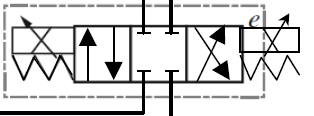
\includegraphics[width=.5\linewidth]{fig_80_cor_01}
%\textit{}
\end{center}
\end{corrige}
\else\begin{marginfigure}
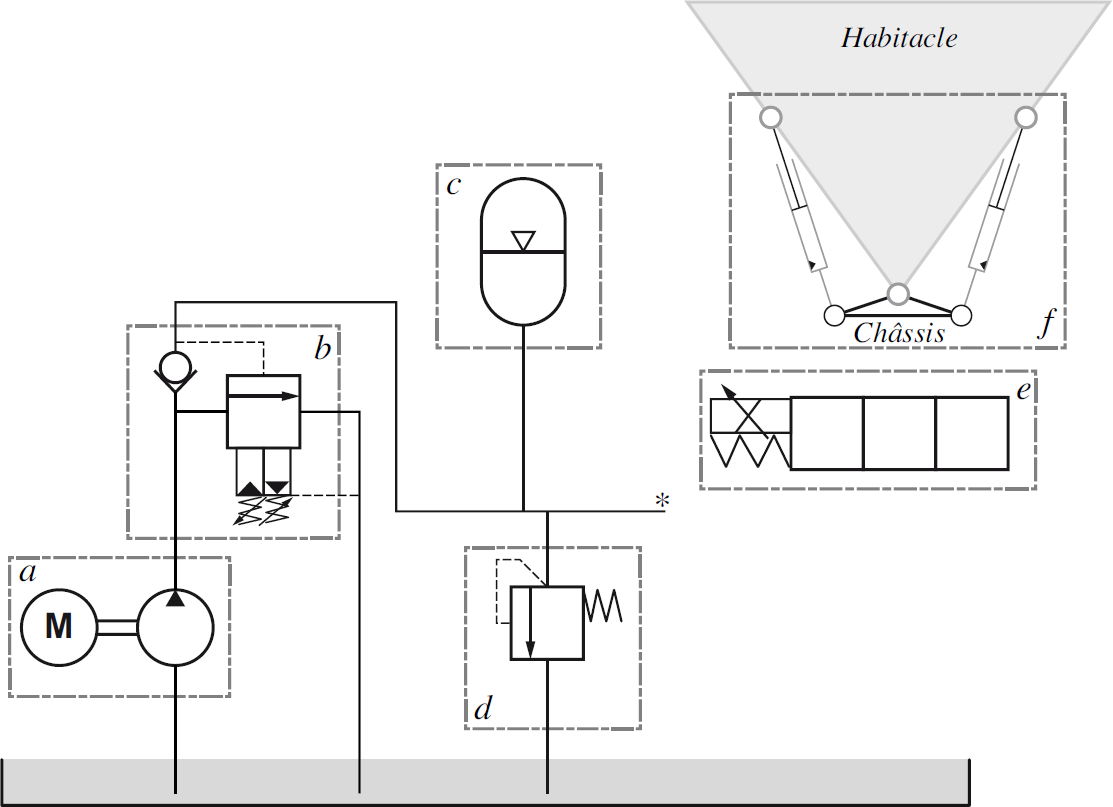
\includegraphics[width=\linewidth]{fig_80_05}
%\textit{}
\end{marginfigure}

\fi

Au démarrage du véhicule, la valve de décharge du module (b) est fermée. Le distributeur à effet proportionnel(e) est en position médiane, les vérins sont donc immobiles. La commande des vérins est initialement bloquée par une temporisation.

\question{En considérant les conditions initiales évoquées, expliquer, en commençant à l’instant de démarrage de la pompe, le comportement du circuit hydraulique en précisant clairement les différentes phases de fonctionnement. Quel est l’utilité de la temporisation ? On souhaite remplacer cette temporisation par un capteur. Préciser la grandeur qu’il devra mesurer. Donner un avantage et un inconvénient du remplacement de la temporisation par ce capteur.}
\ifprof
\begin{corrige}
Démarrage de la pompe et montée en pression du circuit avec remplissage de l’accumulateur (c).

À la fin de la temporisation le distributeur peut être commandé et ainsi alimenter les vérins.

Si la pression augmente trop, alors le limiteur de pression (d) renvoie une partie du fluide vers le
réservoir et si c’est insuffisant alors (b) permet une décharge du circuit (ouverture vers le réservoir
jusqu’à atteindre ne niveau bas réglé).

La temporisation permet d’attendre qu’un niveau de pression suffisant dans le circuit soit atteint.

Pour remplacer la temporisation on peut mesurer la pression dans le circuit ou plus simplement détecter
le niveau de pression satisfaisant pour le fonctionnement à l’aide d’un pressostat.

La solution utilisant un capteur de pression est plus sûre que la temporisation qui pourrait autoriser la
commande du distributeur alors que la pression dans le circuit est encore insuffisante.

(UPSTI). 
\end{corrige}
\else
\fi






\ifprof
\else
\begin{flushright}
\footnotesize{Corrigé  voir \ref{A3:05:80}.}
\end{flushright}%
\fi 
 
\graphicspath{{\repStyle/png/}{../SYS/SYS-01/SYS-01_ChainePuissance/88_Suspension/images/}} 
\normaltrue \difficilefalse \tdifficilefalse
\correctionfalse

%\UPSTIidClasse{11} % 11 sup, 12 spé
%\newcommand{\UPSTIidClasse}{12}
% ATS 2019
\exer{Suspension pneumatique de véhicule de transport routier $\star$ \label{A3:05:88}\label{SYS-01:A3:05:88}}
\setcounter{question}{0}
\marginnote{\xpComp{SYS}{01}}
\index{Compétence A3-05}
\index{Compétence SYS-01}
\index{Suspension pneumatique}
\index{Caractériser un constituant de la chaîne de puissance.}
\index{Distributeur}
\index{Vérin}
\ifcorrection
\else
\marginnote{\textbf{Pas de corrigé pour cet exercice.}}
\fi



\ifprof
\else
La suspension assure la liaison élastique entre le châssis et les essieux. Elle permet principalement d’atténuer les accélérations verticales dues aux variations de profil de la chaussée, contribuant ainsi à l’amélioration du confort et à une meilleure tenue de route.

\begin{marginfigure}
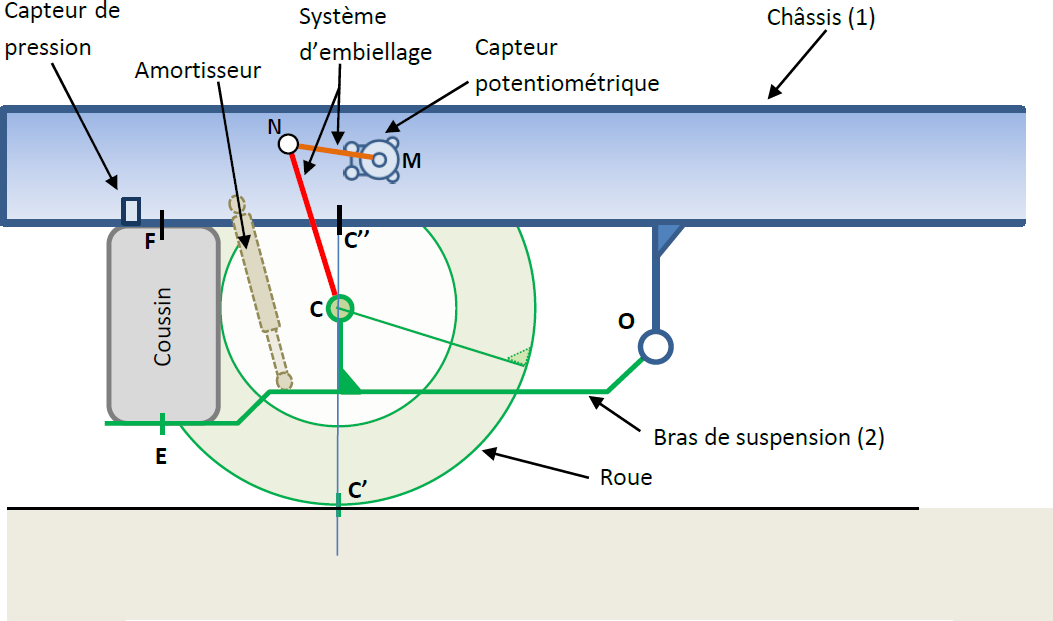
\includegraphics[width=\linewidth]{88_fig_01}
%\textit{}
\end{marginfigure}

Chaque roue possède une suspension pneumatique sur coussin pilotée par des électrovannes, en fonction de données mesurées par des capteurs de pression et des capteurs de position. Un calculateur envoie des commandes électriques aux électrovannes en fonction des besoins.

\begin{marginfigure}
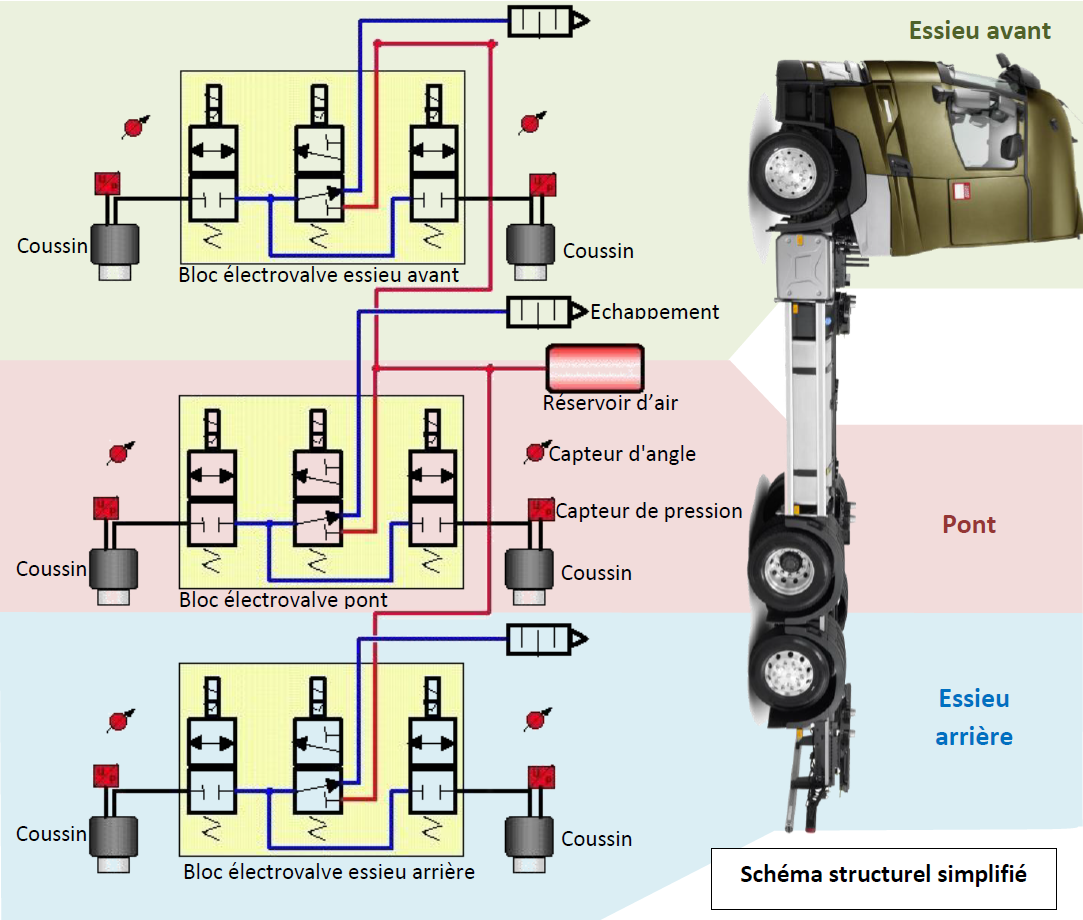
\includegraphics[width=\linewidth]{88_fig_02}
%\textit{}
\end{marginfigure}


\begin{marginfigure}
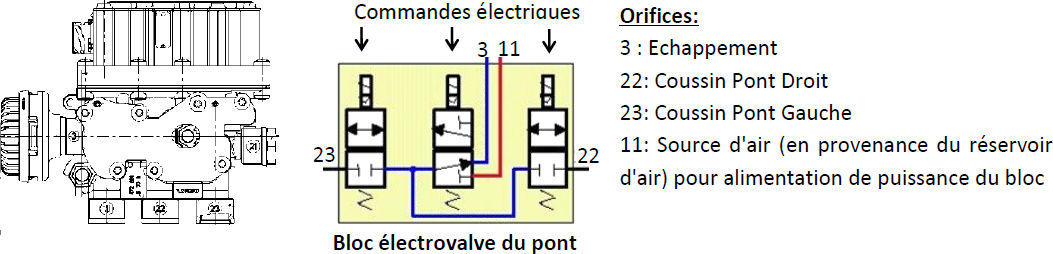
\includegraphics[width=\linewidth]{88_fig_03}
%\textit{}
\end{marginfigure}

Lorsque le niveau mesuré est inférieur à la valeur de consigne (niveau du châssis par rapport au sol), l’électrovalve est commandée de manière à provoquer le gonflage des coussins.
Lorsque le niveau a dépassé la consigne, on commande la vidange des coussins.

\fi
\question{Représenter les trois distributeurs dans la situation de gonflage, puis dans la situation de vidange des coussins.
}
\ifprof
\begin{marginfigure}
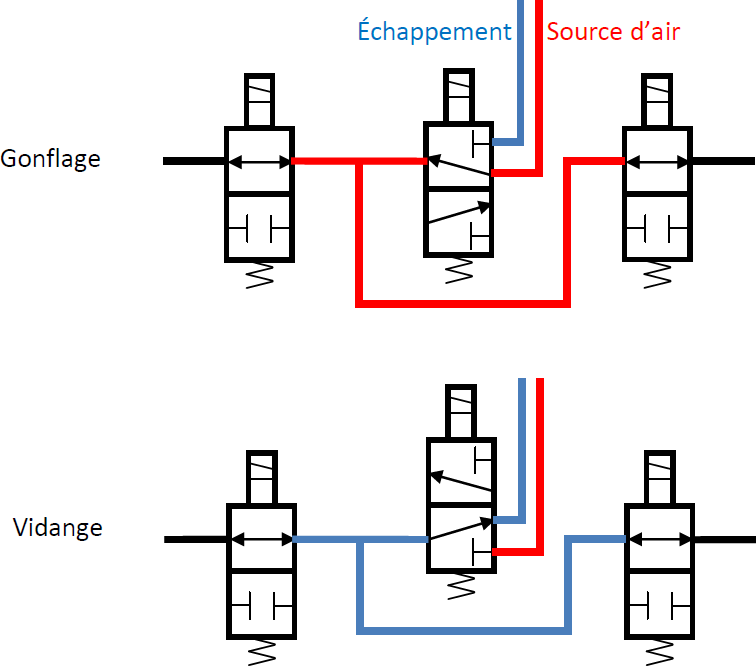
\includegraphics[width=\linewidth]{88_cor_01}
%\textit{}
\end{marginfigure}
\else
\fi

\ifprof
\else
\marginnote{Corrigé  voir \ref{A3:05:88}.}
\fi 
 
\graphicspath{{\repStyle/png/}{../SYS/SYS-01/SYS-01_ChainePuissance/89_Bouee/images/}} 
\normaltrue \difficilefalse \tdifficilefalse
\correctionfalse

%\UPSTIidClasse{11} % 11 sup, 12 spé
%\newcommand{\UPSTIidClasse}{12}
% ATS 2019
\exer{Suspension pneumatique de véhicule de transport routier$\star$ \label{A3:05:89}}
\setcounter{question}{0}
\marginnote{\xpComp{SYS}{01}}%\UPSTIcompetence[2]{A3-05}

\index{Compétence A3-05}
\index{Compétence SYS-01}
\index{Bouée}
\index{Caractériser un constituant de la chaîne de puissance}
\index{Distributeur}
\index{Vérin}
\ifcorrection
\else
\marginnote{\textbf{Pas de corrigé pour cet exercice.}}
\fi



\ifprof
\else
L’énergie produite à partir de la houle est appelée houlomotrice (ou énergie des vagues). Cette énergie est le plus souvent
transformée en énergie électrique.

\begin{marginfigure}
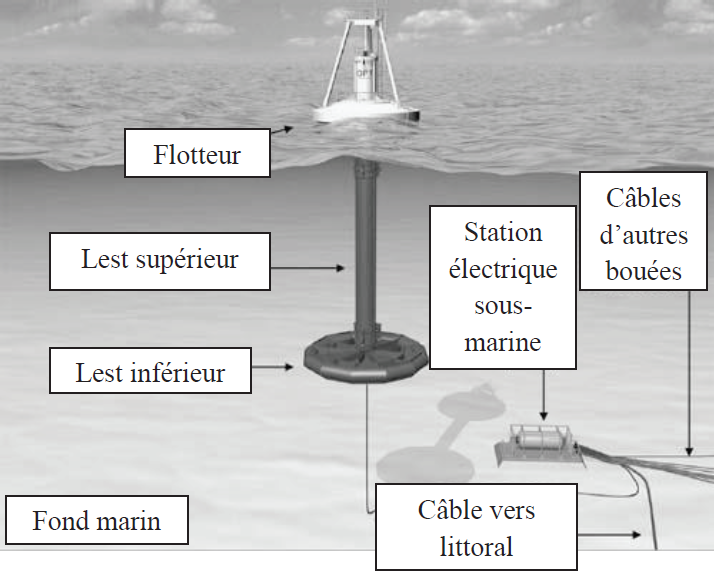
\includegraphics[width=\linewidth]{89_fig_01}
%\textit{}
\end{marginfigure}

Le système de conversion d'énergie est schématisé sur la figue suivante.

Le vérin hydraulique est entraîné par le mouvement relatif de translation entre le flotteur et le lest.
La translation du piston par rapport au cylindre du vérin est donc également paramétrée par le
déplacement $z(t)$ par rapport à la position d’équilibre. La section utile du piston est notée $S_p$. Les
pressions dans les chambres supérieure et inférieure du vérin sont notées respectivement $P_1$ et $P_2$.

Un réservoir accumulateur haute pression (a) et un réservoir accumulateur basse pression (b)
permettent de maintenir les pressions $P_a$ (pression d'admission du moteur hydraulique) et $P_b$
(pression de refoulement du moteur hydraulique) quasi-constantes en régime établi.

Un ensemble de clapets anti-retour permet de générer un débit volumique unidirectionnel $Q_m(t)$
vers le moteur hydraulique, quel que soit le sens de déplacement du piston. Les pertes induites par
ce circuit redresseur seront négligées. On pourra alors considérer en régime établi, et en première
approximation, les relations suivantes entre les pressions dans les réservoirs et dans les chambres du
vérin : $P_a = \text{max} \left(P_1,P_2\right)$ et $P_b = \text{min} \left(P_1,P_2\right)$.

\fi


\question{Compléter les zones en pointillés du schéma hydraulique en dessinant
les clapets anti-retour conformément à la description précédente.}
\ifprof
\begin{corrige}
\begin{center}
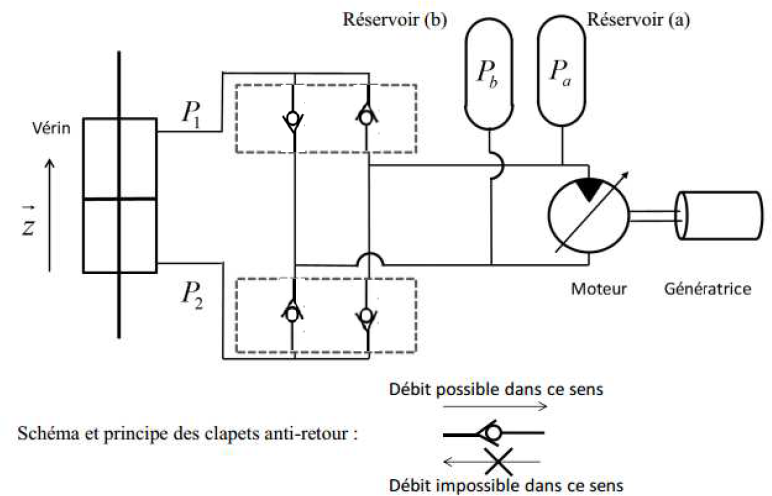
\includegraphics[width=.5\linewidth]{89_cor_01}
%\textit{}
\end{center}
\end{corrige}
\else

\begin{marginfigure}
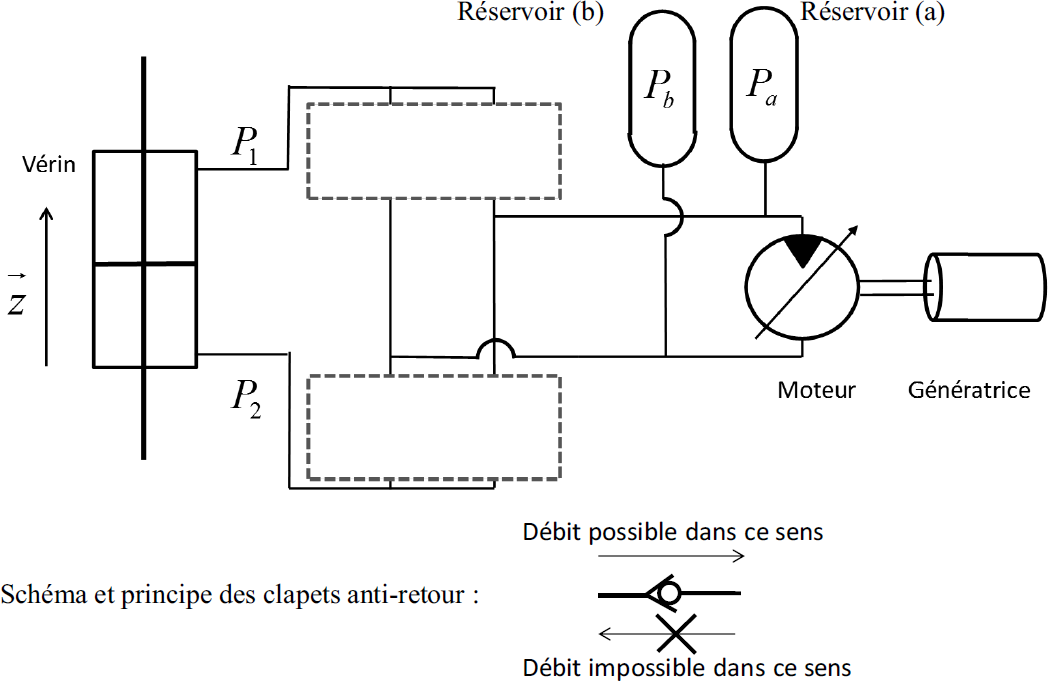
\includegraphics[width=\linewidth]{89_fig_02}
%\textit{}
\end{marginfigure}
\fi

\ifprof
\else
\begin{flushright}
\footnotesize{Corrigé  voir \ref{A3:05:89}.}
\end{flushright}%
\fi 
 
\graphicspath{{\repStyle/png/}{../SYS/SYS-01/SYS-01_ChainePuissance/90_Pilote/images/}} 
\normaltrue \difficilefalse \tdifficilefalse
\correctionfalse

%\UPSTIidClasse{11} % 11 sup, 12 spé
%\newcommand{\UPSTIidClasse}{12}
% ATS 2019
\exer{Pilote hydraulique de voilier $\star$ \label{A3:05:90}}
\setcounter{question}{0}
%\UPSTIcompetence[2]{A3-05}
\xpComp{SYS}{01}
\index{Compétence A3-05}
\index{Compétence SYS-01}
\index{Pilote hydraulique}
\index{Caractériser un constituant de la chaîne de puissance}
\index{Distributeur}
\index{Vérin}
\ifcorrection
\else
\marginnote{\textbf{Pas de corrigé pour cet exercice.}}
\fi



\ifprof
\else
On s'intéresse à la distribution d'énergie hydraulique dans le pilote hydraulique de voilier. 

On donne se premier schéma hydraulique. L'énergie est distribuée par un distributeur monostable 2 positions, 2 orifices. 

\begin{marginfigure}
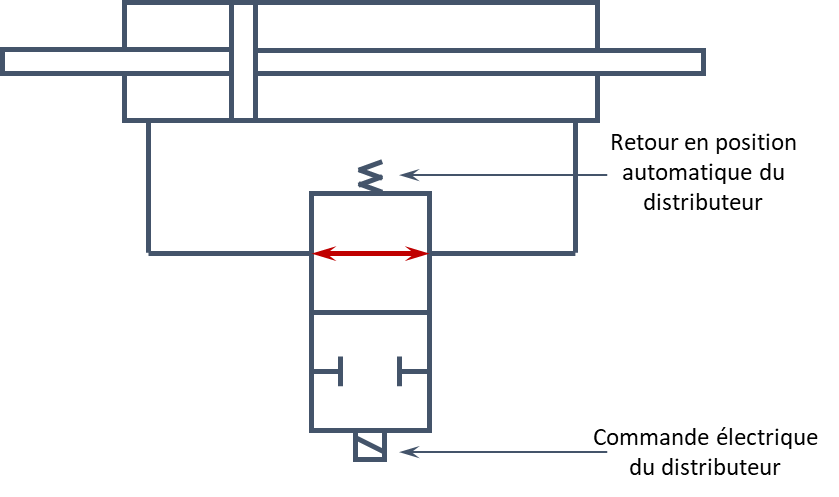
\includegraphics[width=\linewidth]{90_fig_01}
%\textit{}
\end{marginfigure}


\fi


\question{Le schéma précédent est donné dans la situation << au repos >>. Que se passe-t-il si l'utilisateur manipule le vérin à la main ?}
\ifprof
\begin{corrige}
L'huile peut circuler d'une chambre à l'autre en passant par le distributeur. Le vérin peut donc se translater.
\end{corrige}
\else
\fi

\question{On actionne le distributeur. Que se passe-t-il si l'utilisateur manipule le vérin à la main ?}
\ifprof
\begin{corrige}
Le distributeur bloque la circulation de l'huile. Le vérin est bloqué.
%\begin{center}
%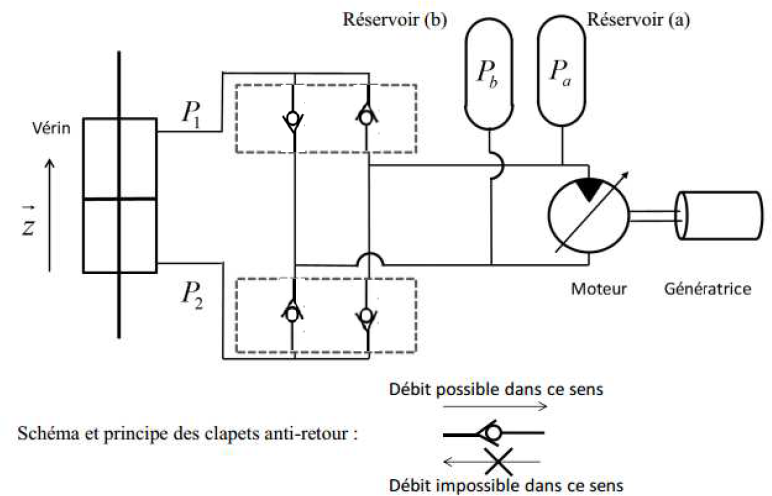
\includegraphics[width=.5\linewidth]{89_cor_01}
%\textit{}
%\end{center}
\end{corrige}
\else
\fi

On complète le schéma avec une motopompe.
\begin{marginfigure}
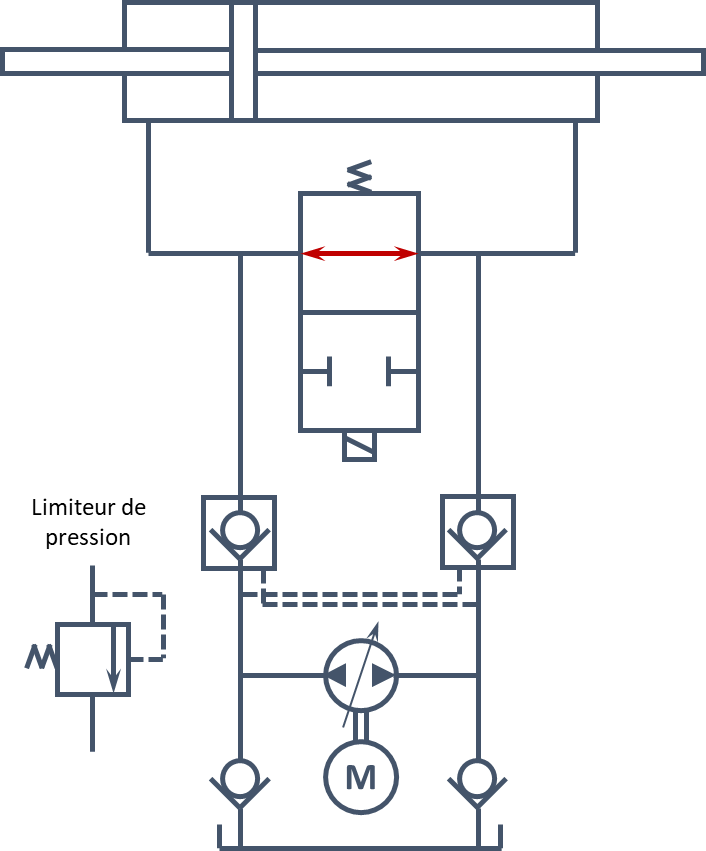
\includegraphics[width=\linewidth]{90_fig_02}
%\textit{}
\end{marginfigure}

\question{On considère le distibuteur activé. Indiquer le sens de fluide permettant de déplacer la tige du vérin vers la gauche. Constatez-vous un problème ?}



\question{Les traits pointillés indiquent un auto-pilotage. Expliquez alors la circulation du fluide ?}


\question{On désire déplacer le vérin vers la gauche, mais la tige est bloquée. Que se passe-t-il ?}

\question{Pour résoudre le problème précédent, on peut utiliser un limiteur de pression. Ajouter le limiteur de pression pour résoudre le problème précédent.}
\ifprof
\else
\begin{flushright}
\footnotesize{Corrigé  voir \ref{A3:05:90}.}
\end{flushright}%
\fi 
 
\section{Analyser une solution technologique} 
\section{Analyser un cahier des charges} 
\section{Valider les performances d'un système vis-à-vis d'un cahier des charges} 
\section{Analyser les résultats d'une simulation ou d'une expérimentation} 
\section{Mesurer et analyser une grandeur physique} 
\setchapterpreamble[u]{\margintoc} 
\chapter{Résoudre un problème de cinématique} 
\section{Analyser un mécanisme, justifier des choix des liaisons, réaliser un schéma cinématique paramétré} 
\graphicspath{{\repStyle/png/}{../CIN/CIN-01-ModeliserSchemasCinematiques/01_T/images/}} 
\normaltrue
\correctiontrue

%\UPSTIidClasse{11} % 11 sup, 12 spé
%\newcommand{\UPSTIidClasse}{12}


\exer{Mouvement T -- $\star$ \label{CIN:01:B2:12:01}}
\setcounter{question}{0}\marginnote{\xpComp{CIN}{01}}%\UPSTIcompetence{B2-12}
\index{Compétence B2-12}\index{Compétence CIN-01}
\index{Mécanisme à 1 translation}
\ifcorrection
\else
\marginnote{\textbf{Pas de corrigé pour cet exercice.}}
\fi

\ifprof
\else
Soit le mécanisme suivant. On note $\vect{AB}=\lambda(t)\vect{i_0}$.
\begin{marginfigure}
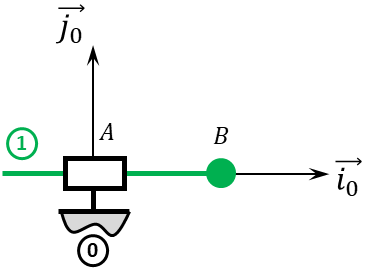
\includegraphics[width=\linewidth]{01_T_01}
\end{marginfigure}
\fi

\question{Tracer le graphe des liaisons.}
\ifprof\begin{marginfigure}
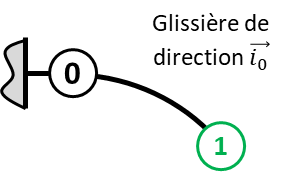
\includegraphics[width=\linewidth]{01_T_01_c}
\end{marginfigure}
\else
\fi


\question{Retracer le schéma cinématique pour $\lambda=\SI{10}{mm}$.}
\ifprof
\begin{marginfigure}
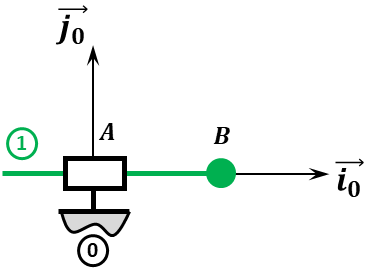
\includegraphics[width=\linewidth]{01_T_02_c}
\end{marginfigure}
\else
\fi

\question{Retracer le schéma cinématique pour $\lambda=-\SI{20}{mm}$.}
\ifprof
\begin{marginfigure}
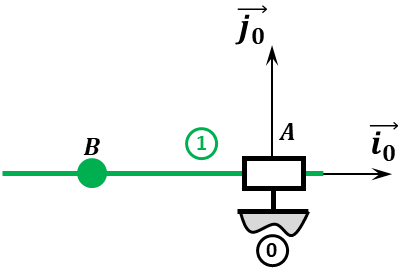
\includegraphics[width=\linewidth]{01_T_03_c}
\end{marginfigure}
\else
\fi

\ifprof
\else
\marginnote{Corrigé  voir \ref{CIN:01:B2:12:01}.}
\fi


 
 
\graphicspath{{\repStyle/png/}{../CIN/CIN-01-ModeliserSchemasCinematiques/02_R/images/}} 
\normaltrue
\correctiontrue

%\UPSTIidClasse{11} % 11 sup, 12 spé
%\newcommand{\UPSTIidClasse}{12}

%\section{Rotation simple} %\label{CIN:01:B2:12:01}
\exer{Mouvement R  $\star$ \label{CIN:01:B2:12:02}}
\setcounter{question}{0}\marginnote{\xpComp{CIN}{01}}%\UPSTIcompetence{B2-12}
\index{Compétence B2-12}\index{Compétence CIN-01}
\index{Mécanisme à 1 rotation}
\ifcorrection
\else
\marginnote{\textbf{Pas de corrigé pour cet exercice.}}
\fi

\ifprof
\else
Soit le mécanisme suivant. On a $\vect{AB}=R\vect{i_1}$ avec $R=\SI{20}{mm}$. 
\begin{marginfigure}
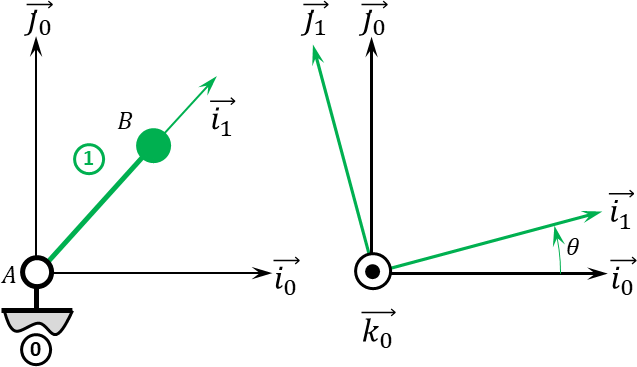
\includegraphics[width=\linewidth]{02_R_01}
\end{marginfigure}
\fi

\ifprof
\begin{multicols}{3}
\else
\fi
\question{Tracer le graphe des liaisons.}
\ifprof
\begin{marginfigure}
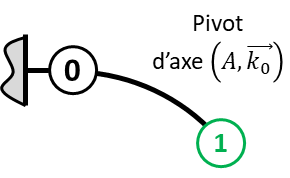
\includegraphics[width=\linewidth]{02_R_01_c}
\end{marginfigure}
\vfill\null
\columnbreak
\else
\fi

\question{Retracer le schéma cinématique pour $\theta=\dfrac{\pi}{4}\,\text{rad}$.}
\ifprof
\begin{marginfigure}
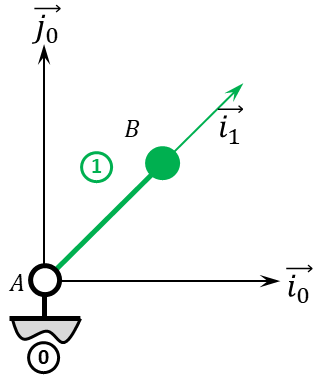
\includegraphics[width=.4\linewidth]{02_R_02_c}
\end{marginfigure}
\vfill\null
\columnbreak
\else
\fi

\question{Retracer le schéma cinématique pour $\theta={\pi}\, \text{rad}$.}
\ifprof
\begin{marginfigure}
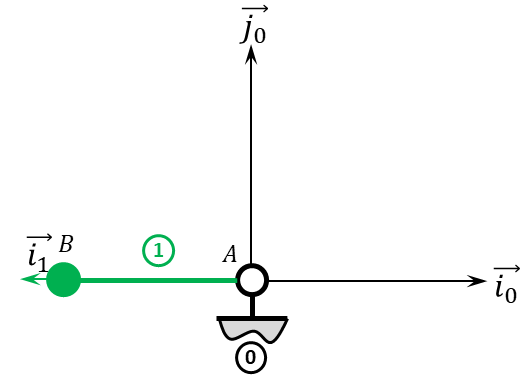
\includegraphics[width=.8\linewidth]{02_R_03_c}
\end{marginfigure}
\else
\fi



\ifprof
\end{multicols}
\else
\fi

\ifprof
\else

\marginnote{Corrigé  voir \ref{CIN:01:B2:12:02}.}

\fi 
 
\graphicspath{{\repStyle/png/}{../CIN/CIN-01-ModeliserSchemasCinematiques/03_TT/images/}} 
\normaltrue
\correctiontrue

%\UPSTIidClasse{11} % 11 sup, 12 spé
%\newcommand{\UPSTIidClasse}{12}


\exer{Mouvement TT -- $\star$ \label{CIN:01:B2:12:03}}
\setcounter{question}{0}\marginnote{\xpComp{CIN}{01}}%\UPSTIcompetence{B2-12}
\index{Compétence B2-12}\index{Compétence CIN-01}
\index{Mécanisme à 2 translations}
\ifcorrection
\else
\marginnote{\textbf{Pas de corrigé pour cet exercice.}}
\fi

\ifprof
\else
Soit le mécanisme suivant. On note $\vect{AB}=\lambda(t)\vect{i_0}$ et $\vect{BC}=\mu(t)\vect{j_0}$.
\begin{marginfigure}
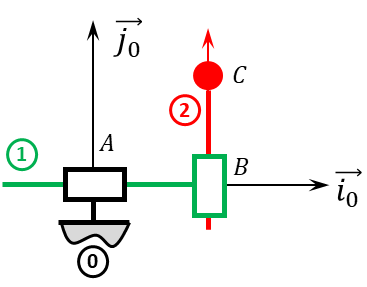
\includegraphics[width=\linewidth]{03_TT_01}
\end{marginfigure}
\fi

\ifprof
\begin{multicols}{3}
\else
\fi
\question{Tracer le graphe des liaisons.}
\ifprof
\begin{marginfigure}
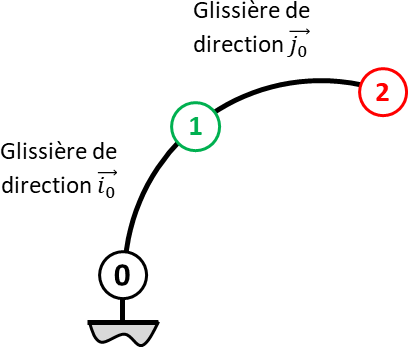
\includegraphics[width=\linewidth]{03_TT_01_c}
\end{marginfigure}
\else
\fi

\question{Retracer le schéma cinématique pour $\lambda=\SI{10}{mm}$ et $\mu=\SI{10}{mm}$.}
\ifprof
\begin{marginfigure}
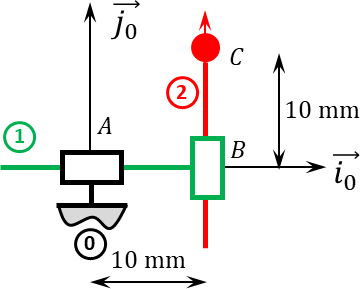
\includegraphics[width=\linewidth]{03_TT_02_c}
\end{marginfigure}
\else
\fi

\question{Retracer le schéma cinématique pour $\lambda=\SI{20}{mm}$ et $\mu=\SI{10}{mm}$.}
\ifprof
\begin{marginfigure}
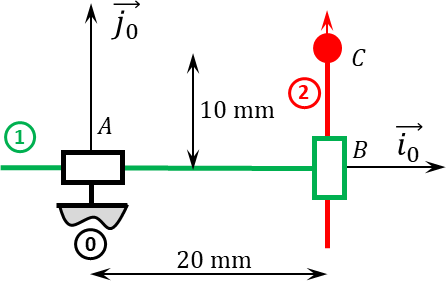
\includegraphics[width=.8\linewidth]{03_TT_03_c}
\end{marginfigure}
\else
\fi


\ifprof
\end{multicols}
\else
\fi

\ifprof
\else

\marginnote{Corrigé  voir \ref{CIN:01:B2:12:03}.}

\fi


 
 
\graphicspath{{\repStyle/png/}{../CIN/CIN-01-ModeliserSchemasCinematiques/04_RR/images/}} 
\normaltrue
\correctiontrue

%\UPSTIidClasse{11} % 11 sup, 12 spé
%\newcommand{\UPSTIidClasse}{12}

\exer{Mouvement RR  $\star$ \label{CIN:01:B2:12:04}}
\setcounter{question}{0}\marginnote{\xpComp{CIN}{01}}%\UPSTIcompetence{B2-12}
\index{Compétence B2-12}\index{Compétence CIN-01}
\index{Mécanisme à 2 rotations}
\ifcorrection
\else
\marginnote{\textbf{Pas de corrigé pour cet exercice.}}
\fi

\ifprof
\else
Soit le mécanisme suivant. On a $\vect{AB}=R\vect{i_1}$ avec $R=\SI{20}{mm}$ et  
$\vect{BC}=L\vect{i_2}$ avec $L=\SI{15}{mm}$.
\begin{marginfigure}
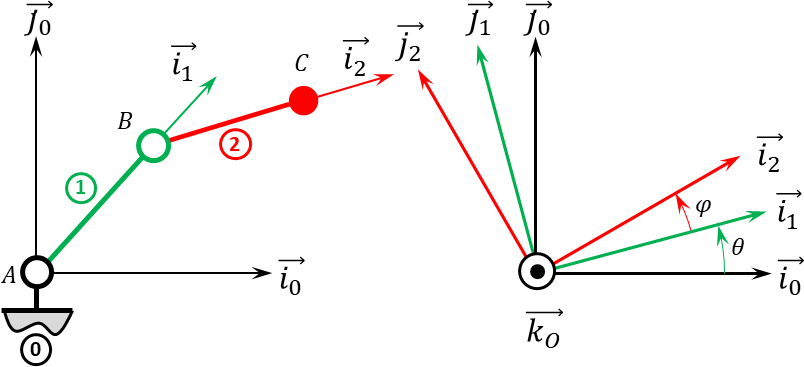
\includegraphics[width=\linewidth]{04_RR_01}
\end{marginfigure}
\fi

\question{Tracer le graphe des liaisons.}
\ifprof
\begin{marginfigure}
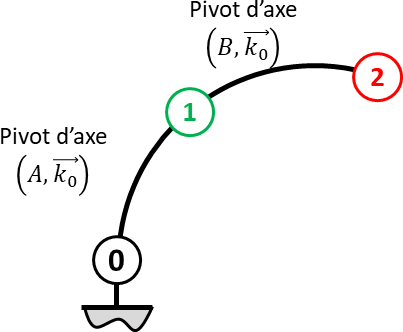
\includegraphics[width=.2\linewidth]{04_RR_01_c}
\end{marginfigure}
\else
\fi


\ifprof
\begin{multicols}{3}
\else
\fi

\question{Retracer le schéma cinématique pour $\theta=\dfrac{\pi}{4}\,\text{rad}$ et $\varphi=\pi\,\text{rad}$.}
\ifprof
\begin{marginfigure}
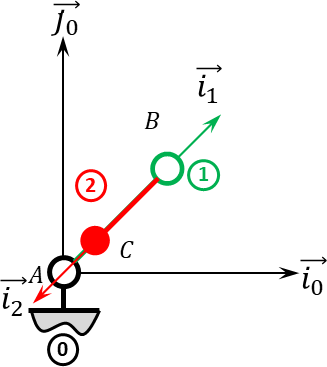
\includegraphics[width=\linewidth]{04_RR_02_c}
\end{marginfigure}
\else
\fi

\question{Retracer le schéma cinématique pour $\theta=\dfrac{\pi}{4}\,\text{rad}$ et $\varphi=-\dfrac{\pi}{4}\,\text{rad}$.}
\ifprof
\begin{marginfigure}
\includegraphics[width=\linewidth]{04_RR_03_c}
\end{marginfigure}
\else
\fi


\question{Retracer le schéma cinématique pour $\theta=\dfrac{3\pi}{4}\,\text{rad}$ et $\varphi=-\dfrac{\pi}{4}\,\text{rad}$.}
\ifprof
\begin{marginfigure}
\includegraphics[width=\linewidth]{04_RR_04_c}
\end{marginfigure}
\else
\fi

\ifprof
\end{multicols}
\else
\fi

\ifprof
\else

\marginnote{Corrigé  voir \ref{CIN:01:B2:12:04}.}

\fi 
 
\graphicspath{{\repStyle/png/}{../CIN/CIN-01-ModeliserSchemasCinematiques/05_RT/images/}} 
\normaltrue
\correctiontrue

%\UPSTIidClasse{11} % 11 sup, 12 spé
%\newcommand{\UPSTIidClasse}{12}

\exer{Mouvement RT  $\star$ \label{CIN:01:B2:12:05}}
\setcounter{question}{0}\marginnote{\xpComp{CIN}{01}}%\UPSTIcompetence{B2-12}
\index{Compétence B2-12}\index{Compétence CIN-01}
\index{Mécanisme à 1 rotation et 1 translation}
\ifcorrection
\else
\marginnote{\textbf{Pas de corrigé pour cet exercice.}}
\fi

\ifprof
\else
Soit le mécanisme suivant. On a $\vect{AB}=\lambda(t)\vect{i_1}$.
\begin{marginfigure}
\includegraphics[width=\linewidth]{05_RT_01}
\end{marginfigure}
\fi

\question{Tracer le graphe des liaisons.}
\ifprof
\begin{marginfigure}
\includegraphics[width=\linewidth]{05_RT_01_01}
\end{marginfigure}
\else
\fi

\question{Retracer le schéma cinématique pour $\theta=\dfrac{\pi}{4}\,\text{rad}$ et $\lambda(t)=\SI{20}{mm}$.}
\ifprof
\else
\fi

\question{Retracer le schéma cinématique pour $\theta=\dfrac{-\pi}{4}\,\text{rad}$ et $\lambda(t)=-\SI{20}{mm}$.}
\ifprof\begin{marginfigure}
\includegraphics[width=.8\linewidth]{05_RT_01_02}
\end{marginfigure}
\else
\fi




\ifprof
\else

\marginnote{Corrigé  voir \ref{CIN:01:B2:12:05}.}

\fi 
 
\graphicspath{{\repStyle/png/}{../CIN/CIN-01-ModeliserSchemasCinematiques/06_TR/images/}} 
\normaltrue
\correctionfalse

%\UPSTIidClasse{11} % 11 sup, 12 spé
%\newcommand{\UPSTIidClasse}{12}

\exer{Mouvement RT  $\star$ \label{CIN:01:B2:12:06}}
\setcounter{question}{0}\marginnote{\xpComp{CIN}{01}}%\UPSTIcompetence{B2-12}
\index{Compétence B2-12}\index{Compétence CIN-01}
\index{Mécanisme à 1 translation et 1 rotation}
\ifcorrection
\else
\marginnote{\textbf{Pas de corrigé pour cet exercice.}}
\fi

\ifprof
\else
Soit le mécanisme suivant. On a $\vect{AB}=\lambda(t)\vect{i_0}$ et $\vect{BC}=R\vect{i2}$.
\begin{marginfigure}
\includegraphics[width=\linewidth]{06_TR_01}
\end{marginfigure}
\fi

\question{Tracer le graphe des liaisons.}
\ifprof
\else
\fi

\question{Retracer le schéma cinématique pour $\theta=\dfrac{\pi}{4}\,\text{rad}$ et $\lambda(t)=\SI{20}{mm}$.}
\ifprof
\else
\fi

\question{Retracer le schéma cinématique pour $\theta=\dfrac{-\pi}{4}\,\text{rad}$ et $\lambda(t)=-\SI{20}{mm}$.}
\ifprof
\else
\fi



\ifprof
\else

\marginnote{Corrigé  voir \ref{CIN:01:B2:12:06}.}

\fi 
 
\graphicspath{{\repStyle/png/}{../CIN/CIN-01-ModeliserSchemasCinematiques/07_RR3D/images/}} 
\normalfalse \difficiletrue \tdifficilefalse
\correctionfalse

%\UPSTIidClasse{11} % 11 sup, 12 spé
%\newcommand{\UPSTIidClasse}{12}

\exer{Mouvement RR 3D  $\star\star$ \label{CIN:01:B2:12:07}}
\setcounter{question}{0}\marginnote{\xpComp{CIN}{01}}%\UPSTIcompetence{B2-12}
\index{Compétence B2-12}\index{Compétence CIN-01}
\index{Mécanisme à 2 rotations 3D}
\ifcorrection
\else
\marginnote{\textbf{Pas de corrigé pour cet exercice.}}
\fi

\ifprof
\else
Soit le mécanisme suivant. On a $\vect{AB}=R\vect{i_1}$ et $\vect{BC}=\ell\vect{i_2}+r\vect{j_2}$. On note $R+\ell=L = \SI{20}{mm}$ et $r=\SI{10}{mm}$.
\begin{marginfigure}
\includegraphics[width=\linewidth]{07_RR3D_01}
\end{marginfigure}
\fi


\question{Tracer le graphe des liaisons.}
\ifprof
\else
\fi

\question{Retracer le schéma cinématique en 3D pour $\theta(t)=\dfrac{\pi}{2}\,\text{rad}$ et $\varphi(t)=\dfrac{\pi}{2}\, \text{rad}$.}
\ifprof
\else
\fi





\ifprof
\else

\marginnote{Corrigé  voir \ref{CIN:01:B2:12:07}.}

\fi 
 
\graphicspath{{\repStyle/png/}{../CIN/CIN-01-ModeliserSchemasCinematiques/08_RR3D/images/}} 
\normalfalse \difficiletrue \tdifficilefalse
\correctionfalse

%\UPSTIidClasse{11} % 11 sup, 12 spé
%\newcommand{\UPSTIidClasse}{12}

\exer{Mouvement RR 3D  $\star\star$ \label{CIN:01:B2:12:08}}
\setcounter{question}{0}\marginnote{\xpComp{CIN}{01}}%\UPSTIcompetence{B2-12}
\index{Compétence B2-12}\index{Compétence CIN-01}
\index{Mécanisme à 2 rotations 3D}
\ifcorrection
\else
\marginnote{\textbf{Pas de corrigé pour cet exercice.}}
\fi

\ifprof
\else
Soit le mécanisme suivant. On a $\vect{AB}=H\vect{j_1}+R\vect{i_1}$ et $\vect{BC}=L\vect{i_2}$. On a $H=\SI{20}{mm}$, $r=\SI{5}{mm}$, $L=\SI{10}{mm}$. 
\begin{marginfigure}
\includegraphics[width=\linewidth]{08_RR3D_01}
\end{marginfigure}
\fi

\question{Tracer le graphe des liaisons.}
\ifprof
\else
\fi

\question{Retracer le schéma cinématique en 3D pour $\theta(t)=\pi\,\text{rad}$ et $\varphi(t)=-\dfrac{\pi}{4}\, \text{rad}$.}
\ifprof
\else
\fi





\ifprof
\else

\marginnote{Corrigé  voir \ref{CIN:01:B2:12:08}.}

\fi 
 
\graphicspath{{\repStyle/png/}{../CIN/CIN-01-ModeliserSchemasCinematiques/09_RT_RSG/images/}} 
\normalfalse \difficiletrue \tdifficilefalse
\correctionfalse

%\UPSTIidClasse{11} % 11 sup, 12 spé
%\newcommand{\UPSTIidClasse}{12}

\exer{Mouvement RT -- RSG  $\star\star$ \label{CIN:01:B2:12:09}}
\setcounter{question}{0}\marginnote{\xpComp{CIN}{01}}%\UPSTIcompetence{B2-12}
\index{Compétence B2-12}\index{Compétence CIN-01}
\index{Mécanisme à 1 rotations, 1 translation et RSG}
\ifcorrection
\else
\marginnote{\textbf{Pas de corrigé pour cet exercice.}}
\fi

\ifprof
\else
Soit le mécanisme suivant. On a $\vect{IA}=R\vect{j_0}$ et $\vect{AB}=\lambda(t)\vect{i_1}$. De plus $R=\SI{15}{mm}$.
\begin{marginfigure}
\includegraphics[width=\linewidth]{09_RT_RSG_01}
\end{marginfigure}
\fi


\question{Tracer le graphe des liaisons.}
\ifprof
\else
\fi


\question{Retracer le schéma cinématique pour $\theta(t)=0\,\text{rad}$ et $\lambda(t)=\SI{20}{mm}$. On notera $I_1$ le point de contact entre \textbf{0} et \textbf{1}.}
\ifprof
\else
\fi

\question{Retracer le schéma cinématique pour $\theta(t)=\dfrac{\pi}{2}\,\text{rad}$ et $\lambda(t)=\SI{30}{mm}$. On notera $I_2$ le point de contact entre \textbf{0} et \textbf{1}. On précisera la position des points $I_{0,0}$ et $I_{0,1}$, points résultants de la rupture de contact lors du passage de $\theta(t)$ de 0 à $\dfrac{\pi}{2}$.}
\ifprof
\else
\fi





\ifprof
\else

\marginnote{Corrigé  voir \ref{CIN:01:B2:12:09}.}

\fi 
 
\graphicspath{{\repStyle/png/}{../CIN/CIN-01-ModeliserSchemasCinematiques/1018_BorneReglable/images/}} 
\normalfalse \difficiletrue \tdifficilefalse
\correctionfalse
%\UPSTIidClasse{11} % 11 sup, 12 spé
%\newcommand{\UPSTIidClasse}{12}

\exer{Borne réglable  $\star\star$ \label{CIN:01:B2:12:1018}}
\setcounter{question}{0}\marginnote{\xpComp{CIN}{01}}%\UPSTIcompetence{B2-12}
\index{Compétence B2-12}\index{Compétence CIN-01}
\index{Schéma cinématique}

\ifcorrection
\else
\marginnote{\textbf{Pas de corrigé pour cet exercice.}}
\fi

\ifprof
\else
Soit la borne réglable suivante. 
\begin{marginfigure}
\includegraphics[width=\linewidth]{1018_01}
\end{marginfigure}
\fi


\ifprof
\else
La nomenclature est la suivante. 

\begin{marginfigure}
\begin{tabular}{lll}
\hline
\textbf{Rep} & \textbf{Désignation} & \textbf{Quantité} \\ \hline 
1 & Coulisseau & 1 \\ 
2 & Borne & 1 \\ 
3 & Corps & 1 \\ 
4 & Vis de guidage & 1 \\ 
5 & Couvercle & 1 \\ 
6 & Vis de couvercle & 2 \\ 
7 & Socle & 1 \\ 
8 & Vis de socle & 4 \\ 
10 & Molette & 1 \\ 
12 & Vis & 1 \\
13 & Goupille fendue & 1 \\ 
\hline
\end{tabular}
\end{marginfigure}
\fi


\question{Colorier le dessin de définition en utilisant la même couleur pour une même classe d'équivalence.}
\ifprof
\else
\fi

\question{Lister les classes classes d'équivalence.}
\ifprof
\else
\fi

\question{Donner le graphe de liaisons en précisant rigoureusement les liaisons. Justifier le choix des liaisons.}
\ifprof
\else
\fi


\question{Réaliser le schéma cinématique.}
\ifprof
\else
\fi

\ifprof
\else

\footnotesize
%\begin{marginfigure}
%\begin{tabular}{|p{.9\linewidth}|}
%\hline
%Indications (à vérifier...) :
%\begin{enumerate}
%\item $\vectv{B}{2}{0} = L\varphip(t)\vj{2} +\thetap(t)\left(L\vj{1}-R\vi{0}\right) $.
%\item  $\torseurcin{V}{2}{0} = \torseurl{\vecto{2}{0}=\left( \varphip(t)+\thetap(t) \right) \vk{0} }{ L\varphip(t)\vj{2} +\thetap(t)\left(L\vj{1}-R\vi{0}\right)}{B}$.
%\item $\vectg{B}{2}{0} =  L\varphipp(t)\vj{2}-L\varphip(t)\left(\varphip(t)+\thetap(t) \right)\vi{2}  + \thetapp(t)\left(L\vj{1}-R\vi{0}\right) - L\thetap^2(t)\vi{1}$.
%\end{enumerate} \\ \hline
%\end{tabular}
%\end{marginfigure}
\normalsize



\marginnote{Corrigé  voir \ref{CIN:01:B2:12:1018}.}

\fi 
 
\graphicspath{{\repStyle/png/}{../CIN/CIN-01-ModeliserSchemasCinematiques/1019_RobotPeinture/images/}} 
\normalfalse \difficiletrue \tdifficilefalse
\correctionfalse
%\UPSTIidClasse{11} % 11 sup, 12 spé
%\newcommand{\UPSTIidClasse}{12}

\exer{Robot de toit  $\star\star$ \label{CIN:01:B2:12:1019}}
\setcounter{question}{0}\marginnote{\xpComp{CIN}{01}}%\UPSTIcompetence{B2-12}
\index{Compétence B2-12}\index{Compétence CIN-01}
\index{Schéma cinématique}

\ifcorrection
\else
\marginnote{\textbf{Pas de corrigé pour cet exercice.}}
\fi

\ifprof
\else
Soit le mécanisme donné au verso.
\fi


\ifprof
\else
La nomenclature est la suivante. 
\begin{multicols}{2}
\begin{marginfigure}
\begin{tabular}{|l|l|l|}
\hline
Rep & Nb  & Désignation \\ \hline \hline % & Matière \\ \hline \hline
1 & 1 & Carter inférieur fixe  \\ \hline %&  Al Si 13 \\ \hline 
2&
1&
Carter supérieur pivotant\\ \hline %& Al Si 13 \\ \hline 
3&
2 &
Ecrou hexagonal ISO 4032 - M10 \\ \hline %& \\ \hline 
4&
1&
Rondelle plate ISO 10673 – Type N - 10 \\ \hline %& \\ \hline 
5&
1&
Axe fileté à tête fendu \\ \hline %& \\ \hline 
6&
1&
Plat de fermeture%&
\\ \hline %S 235 \\ \hline 
7&
7&
Rondelle plate ISO 10673 -- Type N - 5 \\ \hline %& \\ \hline 
8&
1&
Bride de liaison support coussinets \\ \hline % &Al Cu 4 Mg Si \\ \hline 
9&
1&
Bride de liaison gauche \\ \hline % & Al Cu 4 Mg Si   \\ \hline 
10&
2&
Coussinet \\ \hline %& Cu Sn 12 P  \\ \hline 
11&
1&
Tube carter \\ \hline %& \\ \hline 
12&
1&
Bride de liaison droite \\ \hline %& Al Cu 4 Mg Si \\ \hline 
13&
1&
Carter cylindrique\\ \hline % & \\ \hline 
14&
1&
Axe excentré \\ \hline %& \\ \hline 
15&
4&
Vis à tête cylindrique à six pans creux\\ \hline % ISO 4762 - M5-50\\ \hline % & \\ \hline 
16&
1&
Chape mâle\\ \hline % & C 45 \\ \hline 
17&
2&
Goupille cylindrique \\ \hline %ISO 8734 - 2x16 \\ \hline %& \\ \hline 
18&
1&
Bielle rotule \\ \hline % &C 45 \\ \hline 
19&
1&
Cale de réglage \\ \hline %& \\ \hline 
20&
1&
Fermeture rotule \\ \hline %& \\ \hline 
21&
1&
Bielle à portée sphérique \\ \hline %& \\ \hline 
22&
3&
Vis à tête cylindrique à six pans creux  \\
&& ISO 4762 - M5-30 \\ \hline %& \\ \hline 
23&
1&
Goupille cylindrique ISO 8734 - 3x30  \\ \hline %& \\ \hline 
24&
1&
Chape femelle \\ \hline %& \\ \hline %C 45 \\ \hline 

25&
1&
Axe de chape \\ \hline % & \\ \hline 
26&
1&
Anneau élastique pour arbre, 4 x 0,4 \\ \hline % & \\ \hline 
27&
2&
Coussinet à collerette \\ \hline %& Cu Sn 12 P \\ \hline 
28&
1&
Bielle \\ \hline % & C 45 \\ \hline 
\end{tabular}
\end{marginfigure}

\begin{marginfigure}
\begin{tabular}{|l|l|l|}
\hline
Rep & Nb  & Désignation \\ \hline \hline % & Matière \\ \hline \hline
29&
3&
Vis à tête cylindrique à six pans creux \\ \hline % ISO 4762 - M5-18 \\ \hline % & \\ \hline 
30&
1&
Axe d'articulation \\ \hline % & \\ \hline 
31&
1&
Axe de sortie \\ \hline % & \\ \hline %100 Cr 6  \\ \hline 
32&
1&
Support d'axe de sortie \\ \hline %C 45 \\ \hline 
33&
1&
Ecrou hexagonal \\ \hline % ISO 4032 - M24  \\ \hline %& \\ \hline 
34&
1&
Rondelle plate \\ \hline % ISO 10673 – Type S - 24\\ \hline % &  \\ \hline 
35&
2&
Coussinet à collerette \\ \hline %& Cu Sn 12 P  \\ \hline 
36&
1&
Plateau support excentrique \\ \hline %& \\ \hline 
37&
1&
Vis à tête moletée \\ \hline %& \\ \hline 
38&
1&
Doigt de réglage \\ \hline % & C 22 \\ \hline 
39&
1&
Coussinet \\ \hline %& Cu Sn 12 P \\ \hline 
40&
1&
Entretoise  \\ \hline 
41&
2&
Anneau élastique pour arbre, 6 x 0,7  \\ \hline %& \\ \hline 
42&
1&
Anneau élastique pour alésage, 32 x 1,5 \\ \hline %& \\ \hline 
43&
1&
Anneau élastique pour arbre, 12 x 1 \\ \hline %& \\ \hline 
44&
1&
Arbre d’entrée \\ \hline %& \\ \hline 
45&
2&
Roulement à une rangée de \\ 
&& billes à contact radial \\ \hline %& \\ \hline 
46&
1&
Support roulements \\ \hline %& Al Cu 4 Mg Si \\ \hline 
47&
1&
Carter \\ \hline % & Al Cu 4 Mg Si \\ \hline 
48&
1&
Vis sans fin Z48 = 2 filets \\ \hline %& \\ \hline 
49&
2&
Boitier\\ \hline % & \\ \hline 
50&
2&
Roulement à une rangée de \\ 
&& billes à contact radial\\  \hline % & \\ \hline 
51&
2&
Joint à deux lèvres \\ \hline %& \\ \hline 
52&
1&
Arbre Creux\\ \hline % & \\ \hline
53&
1&
Vis à tête hexagonale ISO 4014-M6 \\ \hline %  & \\ \hline 
54 & 
1 &
Arbre \\ \hline % & \\ \hline 
55 &
1&
Roue dentée Z55= 60 dents  \\ \hline %&Cu Ni 2 Si  \\ \hline 
\end{tabular}
\end{marginfigure}

\end{multicols}

\fi

\question{Colorier le dessin de définition en utilisant la même couleur pour une même classe d'équivalence.}
\ifprof
\else
\fi

\question{Lister les classes classes d'équivalence.}
\ifprof
\else
\fi

\question{Donner le graphe de liaisons en précisant rigoureusement les liaisons. Justifier le choix des liaisons.}
\ifprof
\else
\fi


\question{Réaliser le schéma cinématique.}
\ifprof
\else
\fi


\ifprof
\else
\begin{marginfigure}
\includegraphics[width=\linewidth]{1019_01}
\end{marginfigure}
\fi


\ifprof
\else

\footnotesize
%\begin{marginfigure}
%\begin{tabular}{|p{.9\linewidth}|}
%\hline
%Indications (à vérifier...) :
%\begin{enumerate}
%\item $\vectv{B}{2}{0} = L\varphip(t)\vj{2} +\thetap(t)\left(L\vj{1}-R\vi{0}\right) $.
%\item  $\torseurcin{V}{2}{0} = \torseurl{\vecto{2}{0}=\left( \varphip(t)+\thetap(t) \right) \vk{0} }{ L\varphip(t)\vj{2} +\thetap(t)\left(L\vj{1}-R\vi{0}\right)}{B}$.
%\item $\vectg{B}{2}{0} =  L\varphipp(t)\vj{2}-L\varphip(t)\left(\varphip(t)+\thetap(t) \right)\vi{2}  + \thetapp(t)\left(L\vj{1}-R\vi{0}\right) - L\thetap^2(t)\vi{1}$.
%\end{enumerate} \\ \hline
%\end{tabular}
%\end{marginfigure}
\normalsize



\marginnote{Corrigé  voir \ref{CIN:01:B2:12:1018}.}

\fi 
 
\graphicspath{{\repStyle/png/}{../CIN/CIN-01-ModeliserSchemasCinematiques/1020_PompeEnsieta/images/}} 
\normalfalse \difficiletrue \tdifficilefalse
\correctionfalse
%\UPSTIidClasse{11} % 11 sup, 12 spé
%\newcommand{\UPSTIidClasse}{12}

\exer{Pompe ENSIETA  $\star\star$ \label{CIN:01:B2:12:1020}}
\setcounter{question}{0}\marginnote{\xpComp{CIN}{01}}%\UPSTIcompetence{B2-12}
\index{Compétence B2-12}\index{Compétence CIN-01}
\index{Schéma cinématique}
\index{Pompe ENSIETA}

\ifcorrection
\else
\marginnote{\textbf{Pas de corrigé pour cet exercice.}}
\fi



\ifprof
\else
Le plan joint format A4 représente l’ensemble monté d’une pompe hydraulique manuelle.

La pompe est fixée sur un support vertical au moyen de 3 trous filetés (1). Une série de trois trous filetés est usinée sur chaque coté du corps (2), permettant ainsi de fixer indifféremment la pompe sur l’une ou l’autre de ses faces.

L’admission de l’huile est effectuée par l’orifice (3), le refoulement par l’orifice (4).

Le pompage s’effectue en actionnant un levier placé dans l’alésage cannelé du maneton (5). Le mouvement alternatif est, par l’intermédiaire de la biellette articulée, transmis au piston coulissant (6).

Lors du mouvement de droite à gauche du piston coulissant, un volume d’huile est aspiré à travers (3) et vient s’emmagasiner dans l’alésage à droite de la tête du piston, simultanément l’huile qui se trouve à gauche de la tête du piston est refoulée par l’orifice (4).

Lors du mouvement de gauche à droite du piston coulissant s’effectue le transfert, à travers de la tête du piston, de l’huile emmagasinée à sa droite (celle-ci passant côté tige). Simultanément une partie de l’huile transférée est refoulée dans (4).

Un clapet anti-retour est constitué d’une bille et d’un ressort. Sur la pompe étudiée ils sont au nombre de trois. 
Le passage du fluide dans un sens, par action sur la bille provoque l’écrasement du ressort et libère le passage. 
Dans le sens contraire l’action du fluide se conjugue avec celle du ressort et interdit le passage. 
\fi

\question{Le diamètre nominal de la bille contenue dans le clapet anti-retour situé sur l’orifice (4) est identique à celui de l’alésage qui la guide. Est-ce fonctionnellement correct ? Justifier votre réponse. L’observation de la pièce (7) du clapet situé sur l’orifice (3) peut vous aider pour la réponse.}

\question{L’alésage du corps contenant l’extrémité du raccord orifice (4) et l’alésage sur lequel le piston (6) coulisse doivent-ils être réalisés avec le même type d’état de surface ? Justifier votre réponse.}

\question{Entre la tige du piston et l’alésage du corps, quel ajustement choisir ? Préciser s’il s’agit d’un ajustement avec jeu, avec serrage ou ajusté.}

\question{D’après la représentation du dessin d’ensemble, un des composants de la pompe ne peut pas être monté. Quel est-il (donner son numéro) ? Pourquoi ? Que faudrait-il faire pour le rendre montable ?}

\question{Dans le mouvement de droite à gauche du piston, le volume aspiré dans (3) à droite de la tête de piston est-il le même que celui refoulé à gauche de la tête de piston dans (4) ? Justifier votre réponse.}


\ifprof
\else
On donne les dimensions suivantes :
\begin{itemize}
\item tête de piston = \SI{29}{mm};
\item tige de piston = \SI{18}{mm};
\item course du piston = \SI{31}{mm}.
\end{itemize}
\fi

\question{Quel est le volume d’huile  envoyé à la sortie (4) :}
\textit{
\begin{itemize}
\item lors de la course droite -- gauche du piston ?
\item lors de la course gauche -- droite du piston ?
\end{itemize}}


\ifprof
\else

\subsection*{Schéma cinématique}
On considère la pompe sans aucun clapet. Seule la transformation de mouvement permettant le déplacement du piston nous intéresse.

\fi

\question{Faire le schéma cinématique de la pompe.}


\ifprof
\else
\begin{marginfigure}
\includegraphics[width=.9\linewidth]{1020_02}
\end{marginfigure}
\fi


\ifprof
\else

\footnotesize
%\begin{marginfigure}
%\begin{tabular}{|p{.9\linewidth}|}
%\hline
%Indications (à vérifier...) :
%\begin{enumerate}
%\item $\vectv{B}{2}{0} = L\varphip(t)\vj{2} +\thetap(t)\left(L\vj{1}-R\vi{0}\right) $.
%\item  $\torseurcin{V}{2}{0} = \torseurl{\vecto{2}{0}=\left( \varphip(t)+\thetap(t) \right) \vk{0} }{ L\varphip(t)\vj{2} +\thetap(t)\left(L\vj{1}-R\vi{0}\right)}{B}$.
%\item $\vectg{B}{2}{0} =  L\varphipp(t)\vj{2}-L\varphip(t)\left(\varphip(t)+\thetap(t) \right)\vi{2}  + \thetapp(t)\left(L\vj{1}-R\vi{0}\right) - L\thetap^2(t)\vi{1}$.
%\end{enumerate} \\ \hline
%\end{tabular}
%\end{marginfigure}
\normalsize



\marginnote{Corrigé  voir \ref{CIN:01:B2:12:1020}.}

\fi 
 
\graphicspath{{\repStyle/png/}{../CIN/CIN-01-ModeliserSchemasCinematiques/10_PompePalette/images/}} 
\normalfalse \difficiletrue \tdifficilefalse
\correctiontrue

%\UPSTIidClasse{11} % 11 sup, 12 spé
%\newcommand{\UPSTIidClasse}{12}

\exer{Pompe à palettes  $\star\star$ \label{CIN:01:B2:12:10}}
\setcounter{question}{0}\marginnote{\xpComp{CIN}{01}}%\UPSTIcompetence{B2-12}
\index{Compétence B2-12}\index{Compétence CIN-01}
\index{Pompe à palettes}
\ifcorrection
\else
\marginnote{\textbf{Pas de corrigé pour cet exercice.}}
\fi

\ifprof
\else
Soit le mécanisme suivant. On a $\vect{AO}=e\vect{i_0}$ et $\vect{AB}=\lambda(t)\vect{i_1}$. De plus $e=\SI{10}{mm}$ et $R=\SI{20}{mm}$. Le contact entre \textbf{0} et \textbf{2} en $B$ est maintenu en permanence (notamment par effet centrifuge lors de la rotation de la pompe).
\begin{marginfigure}
\includegraphics[width=\linewidth]{10_01}
\end{marginfigure}
\fi


\question{Tracer le graphe des liaisons.}
\ifprof
\begin{marginfigure}
\includegraphics[width=5cm]{10_01_cor}
\end{marginfigure}
\else
\fi


\question{Retracer le schéma cinématique pour $\theta(t)=0 \,\text{rad}$.}
\ifprof
\begin{marginfigure}
\includegraphics[width=5cm]{10_02_cor}
\end{marginfigure}
\else
\fi

\question{Retracer le schéma cinématique pour $\theta(t)=\pi\,\text{rad}$.}
\ifprof
\begin{marginfigure}
\includegraphics[width=5cm]{10_03_cor}
\end{marginfigure}

\else
\fi


\question{En déduire la course de la pièce \textbf{2}.}
\ifprof
La course de la pièce 2 est donnée par la différence entre la longueur $AB$ maximale et $AB$ minimale : $c= 30-10 = \SI{20}{mm}$.
\else
\fi



\ifprof
\else

\marginnote{Corrigé  voir \ref{CIN:01:B2:12:10}.}

\fi 
 
\graphicspath{{\repStyle/png/}{../CIN/CIN-01-ModeliserSchemasCinematiques/11_PompePistonsRadiaux/images/}} 
\normalfalse \difficiletrue \tdifficilefalse
\correctiontrue

%\UPSTIidClasse{11} % 11 sup, 12 spé
%\newcommand{\UPSTIidClasse}{12}

\exer{Pompe à pistons radiaux  $\star\star$ \label{CIN:01:B2:12:11}}
\setcounter{question}{0}\marginnote{\xpComp{CIN}{01}}%\UPSTIcompetence{B2-12}
\index{Compétence B2-12}\index{Compétence CIN-01}
\index{Pompe à pistons radiaux}
\index{Arbre à cames}
\ifcorrection
\else
\marginnote{\textbf{Pas de corrigé pour cet exercice.}}
\fi

\ifprof
\else
Soit le mécanisme suivant. On a $\vect{AB}=e\vect{i_1}$ et $\vect{BI}=R\vect{j_0}$. De plus, 
$e=\SI{10}{mm}$ et $R=\SI{20}{mm}$. Le contact entre \textbf{1} et \textbf{2} en $B$ est maintenu en permanence par un ressort suffisamment raide (non représenté) positionné entre \textbf{0} et \textbf{2}. 
\begin{marginfigure}
\includegraphics[width=\linewidth]{11_01}
\end{marginfigure}
\fi

\question{Tracer le graphe des liaisons.}
\ifprof
\begin{marginfigure}
\includegraphics[width=4cm]{11_01_cor}
\end{marginfigure}
\else
\fi

\question{Retracer le schéma cinématique pour $\theta(t)=0 \,\text{rad}$.}
\ifprof
\else
\fi

\question{Retracer le schéma cinématique pour $\theta(t)=\dfrac{\pi}{2}\,\text{rad}$.}
\ifprof
\else
\fi

\question{Retracer le schéma cinématique pour $\theta(t)=-\dfrac{\pi}{2}\,\text{rad}$.}
\ifprof
\begin{marginfigure}
\includegraphics[width=8cm]{11_02_cor}
\end{marginfigure}
\else
\fi


\question{En déduire la course de la pièce \textbf{2}.}
\ifprof
La course est de 
\else
\fi



\ifprof
\else

\marginnote{Corrigé  voir \ref{CIN:01:B2:12:11}.}

\fi 
 
\graphicspath{{\repStyle/png/}{../CIN/CIN-01-ModeliserSchemasCinematiques/12_BielleManivelle/images/}} 
\normalfalse \difficiletrue \tdifficilefalse
\correctionfalse

%\UPSTIidClasse{11} % 11 sup, 12 spé
%\newcommand{\UPSTIidClasse}{12}

\exer{Système bielle manivelle  $\star\star$ \label{CIN:01:B2:12:12}}
\setcounter{question}{0}\marginnote{\xpComp{CIN}{01}}%\UPSTIcompetence{B2-12}
\index{Compétence B2-12}\index{Compétence CIN-01}
\index{Bielle Manivelle}
\index{Moteur}
\ifcorrection
\else
\marginnote{\textbf{Pas de corrigé pour cet exercice.}}
\fi

\ifprof
\else
Soit le mécanisme suivant. On a $\vect{AB}=R\vect{i_1}$ et $\vect{CB}=L\vect{i_2}$. De plus, 
$R=\SI{10}{mm}$ et $L=\SI{20}{mm}$. 

\begin{marginfigure}
\includegraphics[width=\linewidth]{12_01}
\end{marginfigure}
\fi

\question{Tracer le graphe des liaisons.}
\ifprof
\else
\fi

\question{Retracer le schéma cinématique pour $\theta(t)=\dfrac{\pi}{2}\,\text{rad}$.}
\ifprof
\else
\fi

\question{Retracer le schéma cinématique pour $\theta(t)=-\dfrac{\pi}{2}\,\text{rad}$.}
\ifprof
\else
\fi


\question{En déduire la course de la pièce \textbf{3}.}
\ifprof
\else
\fi



\ifprof
\else
\marginnote{Corrigé  voir \ref{CIN:01:B2:12:12}.}
\fi 
 
\graphicspath{{\repStyle/png/}{../CIN/CIN-01-ModeliserSchemasCinematiques/13_TransfoMouvement/images/}} 
\normalfalse \difficilefalse \tdifficiletrue
\correctionfalse

%\UPSTIidClasse{11} % 11 sup, 12 spé
%\newcommand{\UPSTIidClasse}{12}

\exer{Système de transformation de mouvement  $\star\star$ \label{CIN:01:B2:12:13}}
\setcounter{question}{0}\marginnote{\xpComp{CIN}{01}}%\UPSTIcompetence{B2-12}
\index{Compétence B2-12}\index{Compétence CIN-01}
\index{Bielle Manivelle}
\index{Moteur}
\ifcorrection
\else
\marginnote{\textbf{Pas de corrigé pour cet exercice.}}
\fi

\ifprof
\else
Soit le mécanisme suivant. On a $\vect{AB}=R\vect{i_1}$ et $\vect{CA}=H\vect{j_0}$. De plus, 
$R=\SI{30}{mm}$ et $H=\SI{40}{mm}$. 

\begin{marginfigure}
\includegraphics[width=\linewidth]{13_01}
\end{marginfigure}
\fi


\question{Tracer le graphe des liaisons.}
\ifprof
\else
\fi

\question{Retracer le schéma cinématique pour $\theta(t)=\dfrac{\pi}{2}\,\text{rad}$.}
\ifprof
\else
\fi

\question{Retracer le schéma cinématique pour $\theta(t)=0\,\text{rad}$.}
\ifprof
\else
\fi

\question{Retracer le schéma cinématique pour $\theta(t)=-\dfrac{\pi}{2}\,\text{rad}$.}
\ifprof
\else
\fi


\question{En déduire la course de la pièce \textbf{3}.}
\ifprof
\else
\fi



\ifprof
\else

\marginnote{Corrigé  voir \ref{CIN:01:B2:12:13}.}

\fi 
 
\graphicspath{{\repStyle/png/}{../CIN/CIN-01-ModeliserSchemasCinematiques/14_Sympact/images/}} 
\normalfalse \difficiletrue \tdifficilefalse
\correctiontrue

%\UPSTIidClasse{11} % 11 sup, 12 spé
%\newcommand{\UPSTIidClasse}{12}

\exer{Barrière Sympact $\star\star$ \label{CIN:01:B2:12:14}}
\setcounter{question}{0}\marginnote{\xpComp{CIN}{01}}%\UPSTIcompetence{B2-12}
\index{Compétence B2-12}\index{Compétence CIN-01}
\index{Barrière Sympact}
\ifcorrection
\else
\marginnote{\textbf{Pas de corrigé pour cet exercice.}}
\fi

\ifprof
\else
Soit le mécanisme suivant. On a $\vect{AC}=H\vect{j_0}$ et $\vect{CB}=R\vect{i_1}$. De plus, 
$H=\SI{120}{mm}$ et $R=\SI{40}{mm}$. 

\begin{marginfigure}
\includegraphics[width=\linewidth]{14_01}
\end{marginfigure}
\fi


\question{Tracer le graphe des liaisons.}
\ifprof
\begin{marginfigure}
\includegraphics[width=.4\linewidth]{14_02_c}
\end{marginfigure}
\else
\fi

\question{Retracer le schéma cinématique pour $\theta(t)=\dfrac{\pi}{2}\,\text{rad}$.}
\ifprof
\begin{marginfigure}
\includegraphics[width=.5\linewidth]{14_01_c}
\end{marginfigure}

\else
\fi

\question{Retracer le schéma cinématique pour $\theta(t)=75\degres$.}
\ifprof
\else
\fi


\question{Dans l'hypothèse où la pièce \textbf{1} peut faire des tours complets, quelle doit être la longueur minimale de la pièce \textbf{2}.}
\ifprof
Dans cas, dans le pire des cas, $A$, $B$ et $C$ sont alignés (avec $B$ au-dessus de $C$). Il faut donc $AB = AC+CB = \SI{160}{mm}$.
\else
\fi

\question{Dans l'hypothèse où la pièce \textbf{2} fait \SI{12}{cm}, quel sera le débattement maximal de la pièce \textbf{1}.}
\ifprof
Comme je suis paresseux, j'ai réalisé la construction avec geogebra. On mesure \SI{160,8}{\degres}.
\begin{marginfigure}
\rotatebox{90}{\includegraphics[width=.35\linewidth]{14_03_c}}
\end{marginfigure}
\else
\fi

\ifprof
\else
\ifcolle
\else
\marginnote{
\begin{solution}
\begin{enumerate}
\item .
\item .
\item .
\item \SI{160}{mm}.
\item \SI{160,8}{\degres}.
\end{enumerate}
\end{solution}
\fi
Corrigé  voir \ref{CIN:01:B2:12:14}.}
\fi 
 
\graphicspath{{\repStyle/png/}{../CIN/CIN-01-ModeliserSchemasCinematiques/15_SympactGalet/images/}} 
\normalfalse \difficiletrue \tdifficilefalse
\correctionfalse

%\UPSTIidClasse{11} % 11 sup, 12 spé
%\newcommand{\UPSTIidClasse}{12}

\exer{Barrière Sympact $\star\star$ \label{CIN:01:B2:12:15}}
\setcounter{question}{0}\marginnote{\xpComp{CIN}{01}}%\UPSTIcompetence{B2-12}
\index{Compétence B2-12}\index{Compétence CIN-01}
\index{Barrière Sympact}
\ifcorrection
\else
\marginnote{\textbf{Pas de corrigé pour cet exercice.}}
\fi
\ifprof
\else
Soit le mécanisme suivant. On a $\vect{AC}=H\vect{j_0}$ et $\vect{CB}=R\vect{i_1}$. De plus, 
$H=\SI{120}{mm}$, $R=\SI{40}{mm}$ $BI=\SI{10}{mm}$.

\begin{marginfigure}
\includegraphics[width=\linewidth]{15_01}
\end{marginfigure}
\fi

\question{Tracer le graphe des liaisons.}
\ifprof
\else
\fi

\question{Retracer le schéma cinématique pour $\theta(t)=\dfrac{\pi}{2}\,\text{rad}$.}
\ifprof
\else
\fi

\question{Retracer le schéma cinématique pour $\theta(t)=-\dfrac{\pi}{2}\,\text{rad}$.}
\ifprof
\else
\fi


%\question{En déduire la course de la pièce \textbf{3}.}
%\ifprof
%\else
%\fi



\ifprof
\else
\marginnote{Corrigé voir \ref{CIN:01:B2:12:15}.}
\fi 
 
\graphicspath{{\repStyle/png/}{../CIN/CIN-01-ModeliserSchemasCinematiques/16_Poussoir/images/}} 
\normalfalse \difficiletrue \tdifficilefalse
\correctionfalse

%\UPSTIidClasse{11} % 11 sup, 12 spé
%\newcommand{\UPSTIidClasse}{12}

\exer{Poussoir $\star\star$ \label{CIN:01:B2:12:16}}
\setcounter{question}{0}\marginnote{\xpComp{CIN}{01}}%\UPSTIcompetence{B2-12}
\index{Compétence B2-12}\index{Compétence CIN-01}
%\index{Barrière Sympact}
\ifcorrection
\else
\marginnote{\textbf{Pas de corrigé pour cet exercice.}}
\fi

\ifprof
\else
Soit le mécanisme suivant. On a $\vect{AC}=L\vect{i_0}+H\vect{j_0}$. De plus, 
$H=\SI{120}{mm}$, $L=\SI{40}{mm}$.

\begin{marginfigure}
\includegraphics[width=\linewidth]{16_01}
\end{marginfigure}
\fi


\question{Tracer le graphe des liaisons.}
\ifprof
\else
\fi


\question{Retracer le schéma cinématique pour $\theta(t)=\dfrac{\pi}{4}\,\text{rad}$.}
\ifprof
\else
\fi

\question{Retracer le schéma cinématique pour $\theta(t)=-\dfrac{\pi}{4}\,\text{rad}$.}
\ifprof
\else
\fi


%\question{En déduire la course de la pièce \textbf{3}.}
%\ifprof
%\else
%\fi



\ifprof
\else

\marginnote{Corrigé  voir \ref{CIN:01:B2:12:16}.}

\fi 
 
\graphicspath{{\repStyle/png/}{../CIN/CIN-01-ModeliserSchemasCinematiques/17_4Barres/images/}} 
\normalfalse \difficilefalse \tdifficiletrue
\correctionfalse

%\UPSTIidClasse{11} % 11 sup, 12 spé
%\newcommand{\UPSTIidClasse}{12}

\exer{Système 4 barres $\star\star\star$ \label{CIN:01:B2:12:17}} 
\setcounter{question}{0}\marginnote{\xpComp{CIN}{01}}%\UPSTIcompetence{B2-12}
\index{Compétence B2-12}\index{Compétence CIN-01}
\index{Système 4 barres}
\ifcorrection
\else
\marginnote{\textbf{Pas de corrigé pour cet exercice.}}
\fi

\ifprof
\else
On a : 
%\begin{multicols}{2}
\begin{itemize}
\item $\vect{OA} = a \vx{1}-f \vy{1}$ avec $a=\SI{355}{mm}$ et $f=\SI{13}{mm}$;
\item $\vect{AB} = b \vx{2}$ avec $b=\SI{280}{mm}$;
\item $\vect{BC} = -c \vx{3}$ avec $c=\SI{280}{mm}$;
\item $\vect{OC} = -d \vx{0}-e\vy{0}$ avec $d=\SI{89,5}{mm}$ et $e=\SI{160}{mm}$;
\end{itemize}
%\end{multicols}
%a,b,c,d,e,ff = 355,280,280,89.5,160,13

\begin{marginfigure}
\includegraphics[width=\linewidth]{17_01}

\includegraphics[width=\linewidth]{17_02}
\end{marginfigure}
\fi

\question{Tracer le graphe des liaisons.}
\ifprof
\else
\fi

\question{Retracer le schéma cinématique pour $\theta_1(t)=0\,\text{rad}$.}
\ifprof
\else
\fi

\question{Retracer le schéma cinématique pour $\theta_1(t)=-\dfrac{\pi}{2}\,\text{rad}$.}
\ifprof
\else
\fi


\question{En déduire la course angulaire ($\theta_4$) de la pièce \textbf{3}.}
\ifprof
\else
\fi



\ifprof
\else

\marginnote{Corrigé  voir \ref{CIN:01:B2:12:17}.}

\fi 
 
\graphicspath{{\repStyle/png/}{../CIN/CIN-01-ModeliserSchemasCinematiques/18_Maxpid/images/}} 
\normalfalse \difficilefalse \tdifficiletrue
\correctionfalse

%\UPSTIidClasse{11} % 11 sup, 12 spé
%\newcommand{\UPSTIidClasse}{12}

\exer{Maxpid $\star\star\star$ \label{CIN:01:B2:12:18}}
\setcounter{question}{0}\marginnote{\xpComp{CIN}{01}}%\UPSTIcompetence{B2-12}
\index{Compétence B2-12}\index{Compétence CIN-01}
\index{Maxpid}
\ifcorrection
\else
\marginnote{\textbf{Pas de corrigé pour cet exercice.}}
\fi

\ifprof
\else

Soit le schéma suivant. 
\begin{marginfigure}
\includegraphics[width=\linewidth]{18_01}
\end{marginfigure}
\fi

Par ailleurs $a=\SI{107,1}{mm}$, $b=\SI{80}{mm}$, $c=\SI{70}{mm}$, $d=\SI{80}{mm}$. Le pas de la vis est de $\SI{4}{mm}$.


\question{Tracer le graphe des liaisons.}
\ifprof
\else
\fi

\question{Retracer le schéma cinématique pour $\theta(t)=0\,\text{rad}$.}
\ifprof
\else
\fi

\question{Retracer le schéma cinématique pour $\theta(t)=\dfrac{\pi}{2}\,\text{rad}$.}
\ifprof
\else
\fi


\question{En déduire la course de $\lambda$.}
\ifprof
\else
\fi



\ifprof
\else

\marginnote{Corrigé  voir \ref{CIN:01:B2:12:18}.}

\fi 
 
\graphicspath{{\repStyle/png/}{../CIN/CIN-01-ModeliserSchemasCinematiques/46_RR_RSG/images/}} 
\normalfalse \difficiletrue \tdifficilefalse
\correctionfalse

%\UPSTIidClasse{11} % 11 sup, 12 spé
%\newcommand{\UPSTIidClasse}{12}

\exer{Mouvement RR -- RSG  $\star\star$ \label{CIN:01:B2:12:46}}
\setcounter{question}{0}\marginnote{\xpComp{CIN}{01}}%\UPSTIcompetence{B2-12}
\index{Compétence B2-12}\index{Compétence CIN-01}
\index{Mécanisme à 1 rotations, 1 translation et RSG}
\ifcorrection
\else
\marginnote{\textbf{Pas de corrigé pour cet exercice.}}
\fi

\ifprof
\else
Soit le mécanisme suivant. On a $\vect{IA}=R\vect{j_0}$ et $\vect{AB}=L\vect{i_1}$. De plus $R=\SI{15}{mm}$.
\begin{marginfigure}
\includegraphics[width=\linewidth]{46_RR_RSG_01}
\end{marginfigure}
\fi


\question{Tracer le graphe des liaisons.}
\ifprof
\else
\fi


\question{Retracer le schéma cinématique pour $\theta(t)=0\,\text{rad}$ et $\varphi(t)=0\,\text{rad}$. On notera $I_0$ le point de contact entre \textbf{0} et \textbf{1}.}
\ifprof
\else
\fi

\question{Retracer le schéma cinématique pour $\theta(t)=\dfrac{\pi}{2}\,\text{rad}$ et $\varphi(t)=0\,\text{rad}$. On notera $I_1$ le point de contact entre \textbf{0} et \textbf{1}. On précisera la position des points $I_{0,0}$ et $I_{0,1}$, points résultants de la rupture de contact lors du passage de $\theta(t)$ de 0 à $\dfrac{\pi}{2}$.}
\ifprof
\else
\fi


\question{Retracer le schéma cinématique pour $\theta(t)=\dfrac{\pi}{2}\,\text{rad}$ et $\varphi(t)=\dfrac{\pi}{2}\,\text{rad}$.} 
\ifprof
\else
\fi


\ifprof
\else

\marginnote{Corrigé  voir \ref{CIN:01:B2:12:46}.}

\fi 
 
\graphicspath{{\repStyle/png/}{../CIN/CIN-01-ModeliserSchemasCinematiques/513_Divers_Tabouret/images/}} 
\normalfalse \difficiletrue \tdifficilefalse
\correctionfalse

%\UPSTIidClasse{11} % 11 sup, 12 spé
%\newcommand{\UPSTIidClasse}{12}

\exer{Tabouret  $\star\star$ \label{CIN:01:B2:12:513}}
\setcounter{question}{0}\marginnote{\xpComp{CIN}{01}}%\UPSTIcompetence{B2-12}
\index{Compétence B2-12}\index{Compétence CIN-01}

\ifcorrection
\else
\marginnote{\textbf{Pas de corrigé pour cet exercice.}}
\fi

\ifprof
\else
\begin{marginfigure}
\centering
\includegraphics[width=.5\linewidth]{513_01}
\end{marginfigure}
\fi


\question{Proposer un schéma cinématique permettant de modéliser la liaison entre l'assise et le sol.}
\ifprof
\else
\fi

\ifprof
\else

\marginnote{Corrigé  voir \ref{CIN:01:B2:12:513}.}

\fi 
 
\graphicspath{{\repStyle/png/}{../CIN/CIN-01-ModeliserSchemasCinematiques/514_Divers_Tabouret/images/}} 
\normalfalse \difficiletrue \tdifficilefalse
\correctionfalse

%\UPSTIidClasse{11} % 11 sup, 12 spé
%\newcommand{\UPSTIidClasse}{12}

\exer{Tabouret  $\star\star$ \label{CIN:01:B2:12:514}}
\setcounter{question}{0}\marginnote{\xpComp{CIN}{01}}%\UPSTIcompetence{B2-12}
\index{Compétence B2-12}\index{Compétence CIN-01}

\ifcorrection
\else
\marginnote{\textbf{Pas de corrigé pour cet exercice.}}
\fi

\ifprof
\else
\begin{marginfigure}
\centering
\includegraphics[width=.3\linewidth]{514_01}
\end{marginfigure}
\fi


\question{Proposer 3 schémas cinématiques permettant de modéliser les contacts entre le sol et le tabouret.}
\ifprof
\else
\fi

\ifprof
\else

\marginnote{Corrigé  voir \ref{CIN:01:B2:12:514}.}

\fi 
 
\section{Déterminer un vecteur vitesse, un torseur cinématique, un vecteur accélération} 
\section{Déterminer le rapport de transmission d'un transmetteur} 
\section{Déterminer un loi ES cinématique, utiliser l'hypothèse de RSG} 
\section{Évaluer expérimentalement une grandeur cinématique} 
\setchapterpreamble[u]{\margintoc} 
\chapter{Modéliser un mécanisme} 
\section{Analyser un mécanisme en utilisant un graphe de liaisons} 
\section{Simplifier un mécanisme en utilisant une liaison équivalente} 
\section{Évaluer l'hyperstatisme d'un mécanisme} 
\graphicspath{{\repStyle/png/}{../CHS/CHS-03-HS/64_EPAS/images/}} 
\normaltrue \difficilefalse \tdifficilefalse
\correctiontrue
%\UPSTIidClasse{11} % 11 sup, 12 spé
%\newcommand{\UPSTIidClasse}{11}

\exer{Système EPAS $\star$ \label{CHS:03:B2:16:64}}
%% CCP MP 2007
\setcounter{question}{0}\marginnote{\xpComp{CHS}{03}}%\UPSTIcompetence[2]{B2-16}
\index{Compétence CHS-03}\index{Compétence B2-16}

\index{EPAS}
\index{Hyperstatisme}

\ifcorrection
\else
\marginnote{\textbf{Pas de corrigé pour cet exercice.}}
\fi

\ifprof
\else
On s'intéresse à l'échelle pivotante équipant un camion de pompier. On donne un schéma cinématique du système de manoeuvre du parc échelle.
 
\begin{figure}[h!]
\centering
    \begin{subfigure}[c]{0.45\textwidth}
        \centering
        \includegraphics[width=\linewidth]{64_01.png}
    \end{subfigure}%
    \hfill
    \begin{subfigure}[c]{0.45\textwidth}
        \centering
        \includegraphics[width=\linewidth]{64_02.png}
    \end{subfigure}
    %\caption{Caption place holder}
\end{figure}
\fi

\question{Réaliser le graphe des liaisons.}
\ifprof

\begin{center}
\includegraphics[width=10cm]{64_01_cor}
\end{center}

\else 
\fi

\question{Déterminer le degré d’hyperstatisme de ce mécanisme.}
\ifprof
Détermination des mobilités : 
\begin{itemize}
\item rotation de l'ensemble des pièces en rotation autour de $\vect{y}$ grâce à la pivot entre 0 et 1;
\item rotation de la pivot entre 1 et 2 par mouvements opposés des pivots glissant 4--5 et 4'--5';
\item rotation de la pivot entre 2 et 3 par mouvements simultanés des pivots glissant 6--7 et 6'--7'.
\end{itemize}
On a donc $m=3$. 

\textbf{Méthode cinématique : }
\begin{itemize}
\item nombre de cycles : 15 liaisons et 12 solides, $\gamma = L- S + 1 =4$;
\item nombre d'équations cinématiques: $E_c = 6\times 4 = 24$;
\item nombre d'inconnues cinématiques : $I_c = 4 \times 2+ 11 \times 1 = 19$;
\item hyperstaticité : $h=m-I_c + E_c = 3 -19 + 24 = 8$.
\end{itemize}


\textbf{Méthode statique : }
\begin{itemize}
\item nombre d'équations statiques : $E_s = 6\times 11 = 66$;
\item nombre d'inconnues statiques : $I_s = 4 \times 4+ 11 \times 5 = 71$;
\item hyperstaticité : $h=m-E_s + I_s = 3 -66 + 71 = 8$.
\end{itemize}


\else 
\fi

\question{Proposer des modifications qui permettraient de le rendre isostatique.}
\ifprof
On va chercher à rendre le système isostatique tout en conservant une même architecture pour des branches en parallèles.

Dans le cycle 1--2--5--4--1 pris indépendamment du reste du mécanisme on a :
\begin{itemize}
\item $m=1$;
\item $I_c = 1+1+2+1 = 4$;
\item $E_c =6 \times 1$;
\item $h_1 = m-I_c +E_c = 2 -4 +6 =4$. 
\end{itemize}

En remplaçant la pivot entre 1 et 4 par une linéaire annulaire, on ajoute 3 inconnues cinématiques et 1 mobilité. 
On a donc $h_1 = 2$. On peut faire le même changement pour les liaisons 4' -- 5', 2 -- 6, 2 -- 6'.

On a donc :
\begin{itemize}
\item $m=7$
\item nombre de cycles : 15 liaisons et 12 solides, $\gamma = L- S + 1 =4$;
\item nombre d'équations cinématiques: $E_c = 6\times 4 = 24$;
\item nombre d'inconnues cinématiques : $I_c = 4 \times 2+ 7 \times 1+ 4 \times 4 = 31$;
\item hyperstaticité : $h=m-I_c + E_c = 7 -31 + 24 = 0$.
\end{itemize}
  
(Vérifier que les linéaires annulaires n'ajoutent pas des mobiltés supplémentaires...)

\else 
\fi
 
 

\ifprof
\else
\ifcolle
\else
\marginnote[-4cm]{
\begin{solution}
 \begin{enumerate}
\item .
\item $h=8$.
\item .
 \end{enumerate}
\end{solution}} 
\fi

\marginnote{\footnotesize{Corrigé  voir \ref{CHS:03:B2:16:64}.}}
\fi 
 
\graphicspath{{\repStyle/png/}{../CHS/CHS-03-HS/69_TrainA350/images/}} 
\normaltrue \difficilefalse \tdifficilefalse
\correctiontrue
%\UPSTIidClasse{11} % 11 sup, 12 spé
%\newcommand{\UPSTIidClasse}{11}

\exer{ Train avant d'A350 -- 900$\star$ \label{CHS:03:B2:16:69}}
%% CCP MP 2007
\setcounter{question}{0}\marginnote{\xpComp{CHS}{03}}%\UPSTIcompetence[2]{B2-16}
\index{Compétence CHS-03}\index{Compétence B2-16}

\index{Train d'atterrissage A350}
\index{Hyperstatisme}

\ifcorrection
\else
\marginnote{\textbf{Pas de corrigé pour cet exercice.}}
\fi

\ifprof
\else
La configuration du train d’atterrissage de l’avion A350-900 est de type tricycle avec :
\begin{itemize}
\item deux atterrisseurs principaux (gauche et droit) attachés sur la voilure, légèrement à
l’arrière du centre de gravité $G$ de l’avion et de part et d’autre du plan de symétrie
vertical $\left(O, \vect{x}, \vect{z}\right)$ de l'avion. Ils supportent l’essentiel du poids de l’avion ;
\item un atterrisseur auxiliaire situé sous le nez de l’avion, qui assure l’équilibre longitudinal
de l’avion au sol et permet de manoeuvrer.
\end{itemize}
Les atterrisseurs principaux sont équipés de quatre roues chacun, tandis que
l’atterrisseur auxiliaire est équipé de deux roues.



\begin{marginfigure}
\includegraphics[width=\linewidth]{69_01}
\end{marginfigure}

Les mobilités entre les différents éléments de l’avion (roues,
fuselage…) ne sont pas considérées ; ces éléments ne forment donc qu’une seule
classe d’équivalence désignée « avion ».

\fi

On modélise chacune des 8 liaisons au sol par une liaison ponctuelle (sphère-plan).
\question{Réaliser le graphe des liaisons.}
\ifprof
\begin{center}
\includegraphics[width=5cm]{69_01_cor}
\end{center}
\else 
\fi

\question{Déterminer le degré d’hyperstatisme d’une modélisation de la liaison avion-sol
dans laquelle chaque contact roue-sol serait considéré ponctuel.}
\ifprof
La liaison de l'avion avec le sol est assimilabe à une liaison appui-plan de normale $\vect{z}$. Il y a donc 3 mobilités (1 rotation autour de $\vect{z}$, 1 translation selon $\vect{x}$ et 1 translation suivant $\vect{y}$.

En utilisant une méthode statique, on a $h=m-E_s+I_s$ avec : 
\begin{itemize}
\item  $m=3$;
\item $E_s = 1\times 6 = 6$ (on ne peut isoler que l'avion);
\item $I_s = 10 \times 1 = 10$ (8 liaisons ponctuelles avec 1 inconnue statique par liaison).
\end{itemize}
En conséquences, $h = 3-6+10 =7$. 

En utilisant une méthode cinématique, on a $h=m-I_c+E_c$ avec : 
\begin{itemize}
\item  $m=3$;
\item $E_c = \gamma \times 6 = (10-2+1) \times 6 = 54$ (on ne peut isoler que l'avion);
\item $I_c = 10 \times 5 = 50$ (8 liaisons ponctuelles avec 5 inconnues cinématiques par liaison).
\end{itemize}
En conséquences, $h = 3-50+54 =7$. 

\else 
\fi

Pour simplifier l’étude, les actions mécaniques de contact entre chaque atterrisseur et
le sol sont modélisées globalement par un effort ponctuel vertical. Ainsi la modélisation
introduit trois liaisons ponctuelles de normales $(A, \vect{z})$ (atterrisseur
auxiliaire), $(P_g, \vect{z})$ (atterrisseur principal gauche) et $(P_d, \vect{z})$ (atterrisseur principal droit).

\question{Démontrer que ce modèle simplifié est isostatique.}
\ifprof

En utilisant une méthode statique, on a $h=m-E_s+I_s$ avec : 
\begin{itemize}
\item  $m=3$;
\item $E_s = 1\times 6 = 6$ (on ne peut isoler que l'avion);
\item $I_s = 3 \times 1 = 3$.
\end{itemize}
En conséquences, $h = 3-6+3 =0$. 

En utilisant une méthode cinématique, on a $h=m-I_c+E_c$ avec : 
\begin{itemize}
\item  $m=3$;
\item $E_c = \gamma \times 6 = (3-2+1) \times 6 = 12$ (on ne peut isoler que l'avion);
\item $I_c = 3 \times 5 = 15$ (3 liaisons ponctuelles avec 5 inconnues cinématiques par liaison);
\end{itemize}
En conséquences, $h = 3-15+12 =0$. 

\else 
\fi
 
 

\ifprof
\else
\marginnote[-4cm]{
 \begin{solution}
 \begin{enumerate}
\item .
\item $h=7$.
\item $h=0$.
 \end{enumerate}
\end{solution}
 Corrigé  voir \ref{CHS:03:B2:16:69}.}
\fi 
 
\graphicspath{{\repStyle/png/}{../CHS/CHS-03-HS/71_Robovolc/images/}} 
\normaltrue \difficilefalse \tdifficilefalse
\correctiontrue
%\UPSTIidClasse{11} % 11 sup, 12 spé
%\newcommand{\UPSTIidClasse}{11}

\exer{Pince Robovolc  $\star$ \label{CHS:03:B2:16:71}}
%% CCP MP 2007
\setcounter{question}{0}\marginnote{\xpComp{CHS}{03}}%\UPSTIcompetence[2]{B2-16}
\index{Compétence CHS-03}\index{Compétence B2-16}

\index{Robovolc}
\index{Hyperstatisme}

\ifcorrection
\else
\marginnote{\textbf{Pas de corrigé pour cet exercice.}}
\fi


\question{Calculer l'hyperstatisme du modèle plan du mécanisme global de la pince (\autoref{fig_23}).}
\ifprof
Le graphe de liaisons est donné figure suivante. 

\begin{center}
\includegraphics[width=7cm]{71_01_Cor}
\end{center}
\begin{itemize}
\item Dans le plan, on a $m=2$ : mobilité correspondant au serrage de la pièce et rotation de 6 autour de l'axe $\axe{Q}{z_p}$.
\item $I_c = 6\times 1 + 1 \times 1 + 1 \times 3 = 10$ (6 pivots, 1 glissière et 1 ponctuelle dans le plan);
\item $E_c = 3 \times 3 = 9$
\item $h=m-I_c+E_c = 2-10+9 = 1$. 
\end{itemize}
\else
\fi

\ifprof
\else
\begin{figure}[H]
\centering
\includegraphics[width=.45\linewidth]{fig_23a.png}
\includegraphics[width=.45\linewidth]{fig_23b.png}
\caption{Pince utilisée sur le système ROBOVOLC et schéma cinématique associé \label{fig_23}}
\end{figure} 
\fi 

\ifprof
\else
\marginnote{
\begin{solution}
 \begin{enumerate}
\item $h=1$.
%\item $h=8$.
%\item .
 \end{enumerate}
 \end{solution}}

\marginnote{Corrigé  voir \ref{CHS:03:B2:16:71}.}
\fi 
 
\graphicspath{{\repStyle/png/}{../CHS/CHS-03-HS/71_Robovolc_02/images/}} 
\normaltrue \difficilefalse \tdifficilefalse
\correctionfalse
%\UPSTIidClasse{11} % 11 sup, 12 spé
%\newcommand{\UPSTIidClasse}{11}

\exer{Robovolc $\star$ \label{CHS:03:B2:16:71:02}}
%% 
\setcounter{question}{0}\marginnote{\xpComp{CHS}{03}}%\UPSTIcompetence[2]{B2-16}
\index{Compétence CHS-03}\index{Compétence B2-16}

\index{Robovolc}
\index{Hyperstatisme}

\ifcorrection
\else
\marginnote{\textbf{Pas de corrigé pour cet exercice.}}
\fi


\ifprof
\else
On s'intéresse au Robovolc, une plateforme exploratrice de volcans.

\begin{figure}
\centering
\includegraphics[width=.7\linewidth]{71_01.png}
%\includegraphics[width=.45\linewidth]{77_02.png}
\caption{Schéma cinématique de la plateforme du ROBOVOLC \label{fig_23}}
\end{figure} 

\fi



\question{Réaliser le graphe de liaisons.}

\question{Calculer le degré d'hyperstatisme.}

\question{Si le modèle est hyperstatique, modifier le modèle pour le rendre isostatique.}
 

\ifprof
\else

%\noindent\footnotesize
% \fbox{\parbox{.9\linewidth}{
% Éléments de corrigé : 
% \begin{enumerate}
%\item .
%%\item $h=8$.
%\item .
% \end{enumerate}}}
%\normalsize

\begin{flushright}
\footnotesize{Corrigé  voir \ref{CHS:03:B2:16:79}.}
\end{flushright}%
\fi 
 
\graphicspath{{\repStyle/png/}{../CHS/CHS-03-HS/72_Tripteor/images/}} 
\normaltrue \difficilefalse \tdifficilefalse
\correctiontrue
%\UPSTIidClasse{11} % 11 sup, 12 spé
%\newcommand{\UPSTIidClasse}{11}

\exer{Triptéor $\star$ \label{CHS:03:B2:16:72}}
%% CCP MP 2007
\setcounter{question}{0}\marginnote{\xpComp{CHS}{03}}%\UPSTIcompetence[2]{B2-16}
\index{Compétence CHS-03}\index{Compétence B2-16}

\index{Tripteor}
\index{Hyperstatisme}

\ifcorrection
\else
\marginnote{\textbf{Pas de corrigé pour cet exercice.}}
\fi

\ifprof
\else
Le triptéor est un centre d'Usinage Grande Vitesse à architecture parallèle, permettent d'envisager un usinage rapide et précis.


\begin{figure}[H]
\centering
\includegraphics[width=.45\linewidth]{72_01.png}
%\caption{Pince utilisée sur le système ROBOVOLC et schéma cinématique associé \label{fig_23}}
\hfill\includegraphics[width=.45\linewidth]{72_02.png}
%\caption{Pince utilisée sur le système ROBOVOLC et schéma cinématique associé \label{fig_23}}
\end{figure}

\fi

\question{Réaliser le graphe de liaisons.}
\ifprof
\begin{center}
\includegraphics[width=7cm]{72_01_Cor}
\end{center}
\else
\fi

\question{Calculer le degré d'hyperstatisme.}
\ifprof
\begin{itemize}
\item $m=5$ : translations des 3 glissières et rotations des deux dernières pivot;
\item $I_c=15$;
\item $E_c = 12$;
\item $h=m-I_c+E_c = 5 -15 + 12 = 2$.
\end{itemize}
\else
\fi
 

\ifprof
\else
\marginnote[-4cm]{
\begin{solution}
 \begin{enumerate}
\item .
\item $h=2$.
 \end{enumerate}
 \end{solution}
\footnotesize{Corrigé  voir \ref{CHS:03:B2:16:72}.}}%
\fi 
 
\graphicspath{{\repStyle/png/}{../CHS/CHS-03-HS/81_Piaggio/images/}} 
\normaltrue \difficilefalse \tdifficilefalse
\correctionfalse
%\UPSTIidClasse{11} % 11 sup, 12 spé
%\newcommand{\UPSTIidClasse}{11}

\exer{Scooter Piaggio $\star\star$ \label{CHS:03:B2:16:81}}
%% 
\setcounter{question}{0}\marginnote{\xpComp{CHS}{03}}%\UPSTIcompetence[2]{B2-16}
\index{Compétence CHS-03}\index{Compétence B2-16}

\index{Scooter Piaggio}
\index{Hyperstatisme}

\ifcorrection
\else
\marginnote{\textbf{Pas de corrigé pour cet exercice.}}
\fi


\ifprof
\else
On s'intéresse au système direction du scooter Piaggio. 
La pièce 1 est composée des segments $G_1$ -- $O_1$ -- $D_1$.
La pièce 2 est composée des segments $G_2$ -- $O_2$ -- $D_2$.

\begin{figure*}[!h]
\centering
\begin{subfigure}[c]{.3\linewidth}
\centering
\includegraphics[height=4cm]{81_01.png}
\end{subfigure} \hfill
\begin{subfigure}[c]{.3\linewidth}
\centering
\includegraphics[height=4cm]{81_02.png}
\end{subfigure} \hfill
\begin{subfigure}[c]{.3\linewidth}
\centering
\includegraphics[height=5cm]{81_03.png}
\end{subfigure} 
\end{figure*}
\fi

\question{Réaliser le graphe de liaisons du système de direction. On considèrera le sol comme une classe d'équivalence.}
\ifprof
\begin{center}
\includegraphics[width=.6\linewidth]{81_01_cor.png}
\end{center}
\else
\fi

\question{Calculer le degré d'hyperstatisme.}
\ifprof
\ifcolle
\else
\begin{itemize}
\item $h = m -E_s + I_s$ 
\item $m$ : rotation propre des roues 7 et 8 autour de $\vx{1}$, rotation des roues (7+5) et (6+8) autour de $\vy{1}$,  mouvement du parallèlogramme (1 rotatation), si toutes les liaisons pivots sont bloquées, il reste 2 ponctuelles en parallèle par rapport au sol, soit une liaison linéaire rectiligne (4 mobilités). Au final, $m=9$;
\item $E_S =9\times 6 = 54$;
\item $I_S = 10\times 5 + 2 \times 1 = 52$;
\item $h = 9 -54 + 52 = 7$.
\end{itemize}
\fi
\else
\fi
\question{Si le modèle est hyperstatique, modifier le modèle pour le rendre isostatique.}
\ifprof
SI on considère l'ensemble 0,1,2,3,4 : 
\begin{itemize}
\item $h = m -E_s + I_s$ 
\item $m = 1$; 
\item $E_S =4\times 6 = 24$;
\item $I_S = 6\times 5  = 30$;
\item $h = 1 -24 + 30 = 7$. 
\end{itemize}
Tout l'hyperstatisme est donc concentré dans le double parallélogramme. 

On peut remplcer la pivot en $O_1$ par une linéaire annulaire, ce qui supprime 3 inconnues statiques. 
On peut aussi remplaxer les pivots $G_2$ et $D_2$ par des rotules (supprimant ainsi 4 inconnues statiques).
\else
\fi
 

\ifprof
\else
\ifcolle\else
\marginnote{
\begin{solution}
\begin{enumerate}
\item .
\item $h=7$.
\item .
 \end{enumerate}
 \end{solution}
Corrigé  voir \ref{CHS:03:B2:16:81}.}

\fi
\fi 
 
\graphicspath{{\repStyle/png/}{../CHS/CHS-03-HS/82_MAV/images/}} 
\normaltrue \difficilefalse \tdifficilefalse
\correctionfalse
%\UPSTIidClasse{11} % 11 sup, 12 spé
%\newcommand{\UPSTIidClasse}{11}

\exer{Machine à vendanger $\star\star\star$ \label{CHS:03:B2:16:82}}
%% 
\setcounter{question}{0}\marginnote{\xpComp{CHS}{03}}%\UPSTIcompetence[2]{B2-16}
\index{Compétence CHS-03}\index{Compétence B2-16}

\index{Machine à vendanger}
\index{Hyperstatisme}

\ifcorrection
\else
\marginnote{\textbf{Pas de corrigé pour cet exercice.}}
\fi

\ifprof
\else
On s'intéresse à une machine à vendanger.

\begin{figure}[H]
\centering
\includegraphics[width=\linewidth]{82_01.png}
%\includegraphics[width=.45\linewidth]{77_02.png}
%\caption{Pince utilisée sur le système ROBOVOLC et schéma cinématique associé \label{fig_23}}
\end{figure} 

Le vérin V1, est constitué de deux pièces : le corps, $C_1$ en rouge foncé et la tige $T_1$ en rouge pale. 

\fi

\question{Réaliser le graphe de liaisons.}

\question{Calculer le degré d'hyperstatisme.}

\question{Si le modèle est hyperstatique, modifier le modèle pour le rendre isostatique.}
 

\ifprof
\else

%\noindent\footnotesize
% \fbox{\parbox{.9\linewidth}{
% Éléments de corrigé : 
% \begin{enumerate}
%\item .
%%\item $h=8$.
%\item .
% \end{enumerate}}}
%\normalsize

\begin{flushright}
\footnotesize{Corrigé  voir \ref{CHS:03:B2:16:82}.}
\end{flushright}%
\fi 
 
\graphicspath{{\repStyle/png/}{../CHS/CHS-03-HS/83_Roburoc/images/}} 
\normaltrue \difficilefalse \tdifficilefalse
\correctionfalse
%\UPSTIidClasse{11} % 11 sup, 12 spé
%\newcommand{\UPSTIidClasse}{11}

\exer{Roburoc$\star$ \label{CHS:03:B2:16:79}}
%% 
\setcounter{question}{0}\marginnote{\xpComp{CHS}{03}}%\UPSTIcompetence[2]{B2-16}
\index{Compétence CHS-03}\index{Compétence B2-16}

\index{Roburoc}
\index{Hyperstatisme}

\ifcorrection
\else
\marginnote{\textbf{Pas de corrigé pour cet exercice.}}
\fi


\ifprof
\else
On s'intéresse au roburoc, une plateforme exploratrice tout terrain.


\begin{figure*}[!h]
\centering
\begin{subfigure}[c]{.23\linewidth}
\centering
\includegraphics[height=3cm]{79_01.png}
\end{subfigure} \hfill
\begin{subfigure}[c]{.23\linewidth}
\centering
\includegraphics[height=3cm]{79_02.png}
\end{subfigure} \hfill
\begin{subfigure}[c]{.23\linewidth}
\centering
\includegraphics[height=3cm]{79_03.png}
\end{subfigure} 
\begin{subfigure}[c]{.23\linewidth}
\centering
\includegraphics[height=3cm]{79_04.png}
\end{subfigure}
\end{figure*}




\begin{marginfigure}
\centering
\includegraphics[width=\linewidth]{79_05.png}
%\includegraphics[width=.45\linewidth]{77_02.png}
%\caption{Pince utilisée sur le système ROBOVOLC et schéma cinématique associé \label{fig_23}}
\end{marginfigure} 
\fi


\question{Réaliser le graphe de liaisons.}

\question{Calculer le degré d'hyperstatisme.}

\question{Si le modèle est hyperstatique, modifier le modèle pour le rendre isostatique.}
 

\ifprof
\else

%\noindent\footnotesize
% \fbox{\parbox{.9\linewidth}{
% Éléments de corrigé : 
% \begin{enumerate}
%\item .
%%\item $h=8$.
%\item .
% \end{enumerate}}}
%\normalsize

\marginnote{Corrigé  voir \ref{CHS:03:B2:16:79}.}

\fi 
 
\graphicspath{{\repStyle/png/}{../CHS/CHS-03-HS/84_Nacelle/images/}} 
\normaltrue \difficilefalse \tdifficilefalse
\correctionfalse
%\UPSTIidClasse{11} % 11 sup, 12 spé
%\newcommand{\UPSTIidClasse}{11}

\exer{Nacelle articule de grande portée $\star$ \label{CHS:03:B2:16:84}}
%% 
\setcounter{question}{0}\marginnote{\xpComp{CHS}{03}}%\UPSTIcompetence[2]{B2-16}
\index{Compétence CHS-03}\index{Compétence B2-16}

\index{Nacelle}
\index{Hyperstatisme}

\ifcorrection
\else
\marginnote{\textbf{Pas de corrigé pour cet exercice.}}
\fi


\ifprof
\else
On s'intéresse au châssis d'une nacelle articule de grande portée.

\begin{marginfigure}
\centering
\includegraphics[width=\linewidth]{84_01.png}
%\includegraphics[width=.45\linewidth]{77_02.png}
%\caption{Pince utilisée sur le système ROBOVOLC et schéma cinématique associé \label{fig_23}}
\end{marginfigure} 

La nacelle est amenée à évoluer dans des terrains parfois accidentés (chantier, terrain en friche…).
L’objectif est de valider la motricité du châssis par rapport au sol, même sur un terrain accidenté. 
Le châssis possède un essieu avant monté sur un palonnier pilotable par deux vérins.


\begin{marginfigure}
\centering
\includegraphics[width=\linewidth]{84_02.png}
%\includegraphics[width=.45\linewidth]{77_02.png}
%\caption{Pince utilisée sur le système ROBOVOLC et schéma cinématique associé \label{fig_23}}
\end{marginfigure} 


$C_1$, $C_1'$, $C_2$, $C_2'$ sont les centres respectivement des roues avant droite, avant gauche, arrière droite 
et arrière gauche. Les quatre roues sont considérées en liaison ponctuelle parfaite avec le sol. Les 
points de contact sont notés respectivement $F_1$, $F_1'$, $F_2$, $F_2'$.

\fi

\question{Déterminer le degré d’hyperstatisme du modèle sans les vérins et 
indiquer si ce modèle permet ou non de conserver le contact avec chacune des roues quelle que 
soit la forme du terrain.}

\question{Déterminer le degré d’hyperstatisme du modèle en faisant l'hypothèse que chacune des extrèmités du vérin est en liaison rotule (avec le châssis et l'essieu).}



Les vérins ne sont toujours pas pris en compte. 

\question{Etablir la liaison équivalente réalisée par le train avant entre le sol et le châssis. 
Donner chaque étape de la démarche.}


\question{ Donner l’avantage de la solution constructeur par rapport à une solution à 4 roues 
directement sur le châssis et par rapport à une solution à 3 roues directement sur le châssis.}


\question{Donner le rôle des vérins et indiquer selon quels critères ils peuvent être pilotés.}


\ifprof
\else

%\noindent\footnotesize
% \fbox{\parbox{.9\linewidth}{
% Éléments de corrigé : 
% \begin{enumerate}
%\item .
%%\item $h=8$.
%\item .
% \end{enumerate}}}
%\normalsize

\marginnote{Corrigé voir \ref{CHS:03:B2:16:84}.}
\fi 
 
\section{Simplifier un mécanisme pour le rendre isostatique} 
\section{Analyser les conséquences de l'hyperstatisme d'un mécanisme} 
